\documentclass[twoside,11pt,b5paper,twocolumn]{scrbook}
\usepackage{fontspec} % To use a beautiful font
\defaultfontfeatures{RawFeature={+hlig,+clig,+dlig,+cv11,+cv90,+calt,+ccmp,+swsh},%
  Numbers={Proportional,OldStyle},%
  SmallCapsFeatures={RawFeature={+smcp}},}


\usepackage[hidelinks]{hyperref} % check and put cross-references
\usepackage[british]{babel} % hyphenation
\usepackage{xcolor} % have colors
\usepackage{longtable}
\definecolor{marron}{RGB}{60,30,10}
\definecolor{darkblue}{RGB}{0,0,80}
\definecolor{lightblue}{RGB}{80,80,80}
\definecolor{darkgreen}{RGB}{0,80,0}
\definecolor{lightgreen}{RGB}{10,100,20}
\definecolor{darkgray}{RGB}{0,80,0}
\definecolor{darkred}{RGB}{80,0,0}
\definecolor{shadecolor}{rgb}{0.97,0.97,0.97}

\usepackage{wrapfig}
\usepackage{booktabs}
\usepackage{tabularx}
\usepackage{graphicx}
\usepackage{scrlayer-scrpage} % have fancy headers and footers
\usepackage{lettrine} % For dopped capitals
\usepackage{dblfloatfix} % for specifying two-column table placement
\usepackage{fixltx2e} % for fixing two-column table placement
\usepackage[tmargin=2cm, bmargin=3cm,
lmargin=3cm, rmargin=1.5cm,
headheight=1.0cm,
headsep=0.4cm, footskip=1.5cm]{geometry}


\usepackage[final,stretch=10,protrusion=true,expansion=true]{microtype}
\microtypecontext{spacing=nonfrench}

\setmainfont[SmallCapsFont={EB Garamond}]{EB Garamond}
\setkomafont{disposition}{\rmfamily}

\setlength{\parskip}{1.3ex plus 0.2ex minus 0.2ex}


\usepackage{fourier-orns}

\newcommand{\ornamento}{\vspace{2em}\noindent \textcolor{darkgray}{\hrulefill~ \raisebox{-2.5pt}[10pt][10pt]{\leafright \decofourleft \decothreeleft \aldineright \decotwo \floweroneleft \decoone \floweroneright \decotwo \aldineleft\decothreeright \decofourright \leafleft} ~ \hrulefill \\ \vspace{2em}}}
\newcommand{\ornpar}{\noindent \textcolor{darkgray}{ \raisebox{-1.9pt}[10pt][10pt]{\leafright} \hrulefill \raisebox{-1.9pt}[10pt][10pt]{\leafright \decofourleft \decothreeleft \aldineright \decotwo \floweroneleft \decoone}}}
\newcommand{\ornimpar}{\textcolor{darkgray}{\raisebox{-1.9pt}[10pt][10pt]{\decoone \floweroneright \decotwo \aldineleft \decothreeright \decofourright \leafleft} \hrulefill \raisebox{-1.9pt}[10pt][10pt]{\leafleft}}}

\makeatletter
\def\headrule{{\color{darkgray}\raisebox{-2.1pt}[10pt][10pt]{\leafright} \hrulefill \raisebox{-2.1pt}[10pt][10pt]{~~~\decofourleft \decotwo\decofourright~~~} \hrulefill \raisebox{-2.1pt}[10pt][10pt]{ \leafleft}}}
\makeatother

\newcommand{\estcab}[1]{\textsc{\textcolor{marron}{#1}}}

\renewcommand{\chaptermark}[1]{}
\renewcommand{\sectionmark}[1]{}
\lohead{\estcab{\rightmark}}
\rohead{\estcab{\leftmark}}
\lehead{\estcab{\rightmark}}
\rehead{\estcab{\leftmark}}

\ofoot{}
\lofoot{\ornimpar \\ \large \hfill \textcolor{darkgray}{\leafNE ~~~ \textrm{\thepage}}}
\refoot{\ornpar \\ \large \textcolor{darkgray}{\textrm{\thepage} ~~~ \reflectbox{\leafNE}} \hfill}

\newcommand{\keyword}[1]{\textcolor{darkgreen}{#1}}
\renewcommand{\paragraph}[1]{\par\noindent\markboth{#1}{#1}\estcab{\keyword{#1}}\label{#1} }
\newcommand{\see}[1]{{\estcab{\hyperref[#1]{#1}}}}
\newcommand{\proverb}[1]{\par \textcolor{darkblue}{\itshape #1}}

\pagestyle{scrheadings}

\usepackage{chngcntr}
\counterwithout{figure}{chapter}
\counterwithout{table}{chapter}

\begin{document}

\begin{titlepage}
 \centering
 \vspace*{\baselineskip}
 \rule{\textwidth}{1.6pt}\vspace*{-\baselineskip}\vspace*{2pt}
 \rule{\textwidth}{0.4pt}\\[\baselineskip]
 
 {\Huge \itshape Encyclopædia Imperialys;}\\[0.4em]
 {\Large Or,\\[0.4em]}
 {\huge\scshape A Landskeeper's Compendium}\\
 \rule{\textwidth}{0.4pt}\vspace*{-\baselineskip}\vspace{3.2pt}
 \rule{\textwidth}{1.6pt}\\[\baselineskip]
 {\Large on Matters \scshape Magickal, Virtuous, Political {\normalfont and} Mundane,\\[1em]}
 {\itshape Compiled upon a New Plan, such that\\[0.5em]}
 {\large the different Arts and Practices are digested into distinct Essayes or Systems, including helpful Tables}
 
 {\itshape And\\[0.5em]}
 {\large All Technical Terms, \textit{\&c.} are explained as they occur \\[0.5em] \itshape in the Order of the Alphabet.}

 \vspace{0.8cm}
 {\bfseries Illustrated with enlightening Pictures.}
 
 \vfill
 
 Printed for Abbot James of Pickham,\\[0.4em]
 by Robyn Painter in {\itshape Pete’s Virtuous Printing-Office, T'King's Stoke}
 
 {\scshape Anno CCCLXXX}
\end{titlepage}
\begin{uppertitleback}{}
Contributions by James Appleseeder of Pickham, Abbot; t'late Peter Keeper, Cardinal and Landskeeper; Nicholas Reaper, Landskeeper; Martin Orchards, Landskeeper; t'late Annis Ramsbruck; Reinholz, Magistrate; and other members of t'Imperial Civil Service.

This book was written with t'intention to provide Wise and Vigilant ken, and to be an initial resource for any landskeeper looking to solve problems outside their field of expertise. Therefore, further contributions and any fundamental questions left unanswered are welcome.

All text, and all images marked \textit{*}, are published under civil service code \textit{cc-by-sa}, meaning that it will not be held against thee if thou findst this book helpful enough to reproduce any or all of it through other means.

Second edition, 379 YE.
\end{uppertitleback}
\setlength{\parindent}{1em}

\listoftables

\paragraph{abbot} t'\allowbreak head \see{monk} of a \see{monastery}. Often addressed as “father” or “mother”. 
\paragraph{abuse of powers}t'religious \see{crime} of abusing t'\allowbreak powers of a priest. This includes t'\allowbreak powers of t'\allowbreak synod, as well as liao ceremonies.
\paragraph{Alderly} a forested region in central \see{Mournwold}, held by t'\allowbreak \see{jotun}.
\paragraph{aldermen} a representative of a \see{market town}. In most cases these men or women are wealthy merchants of t'\allowbreak town, but often they include prominent town folk such as a \see{friar} or blacksmith who lives in t'\allowbreak village. Those market towns that employ their own militia usually raise t'\allowbreak captain to t'\allowbreak rank of alderman. T'\allowbreak innkeeper is almost invariably an alderman of t'\allowbreak town and can be one of t'\allowbreak wealthiest members of t'\allowbreak community. Many aldermen take great pride in their ceremonial chains of office. Several towns are in competition in providing t'\allowbreak most magnificent chain for their representative, and some go so far as to commission them as \see{magickal item}s, such as an Alderman's Edge. \proverb{Without labor nothing prospers.}
\paragraph{ambergelt} a resin in red or similar colours, generally symbolised by a wasp. Used by \see{magicksmith}s to create \see{magickal item}s that heal, slow or preserve life. Also used for decoration, or as a resinous varnish.
\paragraph{Ambition} a \see{virtue} \proverb{There's never a tree so big it can't be felled.}
\paragraph{amity} (do not confuse with \see{enmity}) means that an \see{eternal} and their \see{herald}s are considered to be \see{foreigner}s, and therefore have t'\allowbreak same protection under t'\allowbreak \see{law} as Imperial \see{citizen}s.
\paragraph{anoint} a priestly ceremony strengthening t'\allowbreak immediate connection between an individual and a \see{virtue} for short time.
\paragraph{Anvil} location of t'\allowbreak \see{sentinel gate} and t'\allowbreak \see{senate} and capital location of t'\allowbreak \see{Empire}. Four times a year t'\allowbreak powerful citizens of t'\allowbreak \see{Empire} meet here to determine t'\allowbreak future of their people. Founded on t'\allowbreak ruins of t'\allowbreak old smithy in which t'\allowbreak \see{first Empress} took shelter from her enemies when a young woman, Anvil is said to be where t'\allowbreak first open declaration of t'\allowbreak dream of \see{Empire} was made. After her ascension to t'\allowbreak throne, t'\allowbreak Empress declared that t'\allowbreak small settlement would be preserved for t'\allowbreak lifetime of t'\allowbreak \see{Empire} in memory of sacrifices made by those sheltering her. Since then Imperial parliaments have been held there, but t'\allowbreak town itself has never been allowed to grow. In addition to t'\allowbreak senate and sentinel gate, Anvil's permanent features are t'\allowbreak Forge (now a pub), t'\allowbreak Imperial \see{regio} and t'\allowbreak site of t'\allowbreak war memorial.%Tyke's eatery (\emph{Dine at Tyke's!}) 
\paragraph{Applewood} a village in \see{Stock March}, founded by a coalition of several \see{household}s after a particularly vicious \see{Feni} attack in t'\allowbreak \allowbreak 370s.
\paragraph{artisan} a skilled craft worker who makes or creates things by hand that may be functional or strictly decorative. Often used synonymously with \see{magicksmith}.
\paragraph{artisan's oil} an oleaginous goop used by \see{magicksmith}s to mend t'\allowbreak structure of broken \see{magickal item}s.
\paragraph{Ashbrook} a region and eponymous river in \see{Upwold}.
\paragraph{assembly} t'\allowbreak individual bodies of t'\allowbreak \see{synod} are referred to as assemblies. T'Marcher assembly, and most \see{virtue} assemblies, welcome interested laypeople such as \see{pilgrim}s of t'\allowbreak way, friars, or priests without a congregation, even though these individuals do not have t'\allowbreak right to vote on judgements.
\paragraph{autumn} 1: a season 2: t'\allowbreak \see{magick}al realm of wealth, bargins and power \proverb{Reap what you sow, come rain, shine or snow.}
\paragraph{bailiff of t'grand market} T'Bailiff of t'\allowbreak grand market is an Imperial title awarded to a Marcher citizen. It is a Marcher position appointed through t'\allowbreak Bourse but chosen by Marcher yeomen with votes allocated based on t'\allowbreak size of their farm holdings. T'Bailiff has offices in Meade, but it is a rare Bailiff who spends much time there. While t'\allowbreak title is associated closely with t'\allowbreak weekly or bi-weekly markets of Mitwold, t'\allowbreak Bailiff is regularly involved in trade fairs and markets across t'\allowbreak Marches, and Marchers from every territory have regularly held t'\allowbreak post. T'title pre-dates t'\allowbreak formation of t'\allowbreak \see{market town}s, and comes from a time when almost every town and village in t'\allowbreak nation would have their own regular market. Traditionally t'\allowbreak Bailiff's role was to ensure security at fairs and markets across t'\allowbreak Marches. In return, they were guaranteed a hearty meal, a minimum of one meat pie and a tankard of ale. More importantly, however, to help t'\allowbreak Bailiff meet t'\allowbreak costs of their office they were given t'\allowbreak opportunity to buy some goods before t'\allowbreak market officially opened allowing shrewd bailiffs to secure bargains for themselves. Many markets considered it a matter of Pride to ensure that t'\allowbreak Bailiff turned a good profit in exchange for their hard work in keeping t'\allowbreak marketplace safe and fair for all. Within t'\allowbreak space of a season, t'\allowbreak Bailiff might find themselves in a position to buy beggar's lye and ambergelt at a fair from a village in t'\allowbreak birchwoods of \see{Upwold}; a cask of Wintermark mead and some measures of \see{dragonbone} from a Suaq peddlar in a town square in \see{Mitwold}; a basket of tempest jade from a scowling stallholder at t'\allowbreak great market in Meade; a basket of assorted herbs at a dour fair in \see{Bregasland} or even a handful of \see{crystal mana} at a strained gathering in Overton. When t'\allowbreak Marches joined t'\allowbreak \see{Empire} some of t'\allowbreak more expensive responsibilities of t'\allowbreak Bailiff were assumed by t'\allowbreak civil service. Marchers are loath to abandon their traditions however; t'\allowbreak presence of an honest Bailiff was considered to be good for trade as it let everyone ken that t'\allowbreak market was safe to travel to. With t'\allowbreak help of Emperor Giovanni t'\allowbreak role of Bailiff was incorporated into t'\allowbreak Bourse, to allow t'\allowbreak \see{civil service} to identify t'\allowbreak individual with t'\allowbreak most support from other yeomen. T'Bailiff is expected to ensure fairs, markets and trade gatherings in t'\allowbreak Marches are undertaken in a traditional and honest fashion. They also have some responsibility for ensuring that t'\allowbreak major roads between towns and villages remain free of bandits and \see{Feni} who might otherwise restrict trade. In practice, this is quite a tall order for a single individual – many markets have their own local bailiff or sheriff who sees to t'\allowbreak security of their fair. Specifically, t'\allowbreak Bailiff oversees t'\allowbreak grand market in Meade which takes place on t'\allowbreak third weekend of each month and attracts traders from across t'\allowbreak Marches and even occasionally from Wintermark to t'\allowbreak north. 
\paragraph{barbarian} anyone with whom t'\allowbreak \see{Empire} is at war, including during a ceasefire. \see{eternal}s and t'\allowbreak \see{herald}s of \see{eternal}s who are t'\allowbreak subject of a declaration of \see{enmity} by t'\allowbreak \see{conclave} are considered enemies of t'\allowbreak \see{Empire} and treated as barbarians. Unauthorised dealings with barbarians are illegal and will be investigated as treason. Any delegations from barbarian nations who arrive on t'\allowbreak field of Anvil under a flag of peace have protection under t'\allowbreak \see{law} as if they were Imperial citizens for t'\allowbreak duration of their visit and for their direct passage out of t'\allowbreak \see{Empire}. Otherwise barbarians have no protection under t'\allowbreak law.\proverb{Where t'hedge is lowest men jump over.}
\paragraph{battle} a fight between many people on each side. In \see{Anvil}, \see{constellation}s usually permit two battles per week facilitated through t'\allowbreak \see{sentinel gate}, involving fighters from five \see{nation}s to pass through t'\allowbreak gate.
\paragraph{beak} t'\allowbreak hard mouth of a bird or herald of \see{Lashonar}.
\paragraph{beater} beaters roam t'\allowbreak Marches, learning every part of t'\allowbreak land, watching for thieves, vagrants and other ne'er-do-wells. Beaters mark out what land belongs to whom.  Beaters are often instrumental in settling land disputes between neighbours and they still play a vital role in t'\allowbreak tradition of t'\allowbreak \see{beating of t'bounds}. T'beating of t'\allowbreak bounds usually takes place after t'\allowbreak harvest is in. At this festival every Marcher marks their land, by walking around t'\allowbreak boundary led by t'\allowbreak beaters. Certain stones, trees or other marker points around t'\allowbreak boundary are beaten literally, ceremonially striking them with sticks or willow wands. T'\see{market town}s beat t'\allowbreak boundaries laid out by their warrant, and individual towners often have a second ceremony in which they beat t'\allowbreak bounds of their shop or workplace. T'ceremony is designed to remind all of t'\allowbreak size of t'\allowbreak holding, but it also works to remind everyone of who is part of t'\allowbreak community and who is outside it. On a practical level, t'\allowbreak beating of t'\allowbreak bounds is often preceded by t'\allowbreak beaters ensuring that t'\allowbreak boundary areas are safe for t'\allowbreak upcoming ceremony, and followed by a period of maintaining and replacing whatever physical markers delineate t'\allowbreak bounds – it is a time for repairing fences, planting hedges and t'\allowbreak like. Beaters often live off t'\allowbreak land and most are skilled woodsmen and hunters. They serve as an informal police force, investigating crimes and tracking criminals. While an individual beater often associates with one or more \see{household}s, they make no secret of t'\allowbreak fact that they maintain an informal network among themselves. T'beaters watch t'\allowbreak boundaries and defend them against trespass until its forces can muster. They also remain vigilant for internal threats. In addition to t'\allowbreak orcs that still occupy t'\allowbreak more inaccessible hills and wild forests of t'\allowbreak Marches, there are bands of \see{Feni} who launch raids against civilised Marchers to steal metal, cattle or crops. If something or someone is raiding out of t'\allowbreak forests or hills then t'\allowbreak beaters are t'\allowbreak ones who are called on to hunt it. T'third Marcher army, t'\allowbreak \see{bounders} of \see{Upwold}, contains a large number of beaters.
\paragraph{beater's gate} A wayhouse south of \see{Greywater}, kent for its hospitability, in particular to travelling \see{beater}s. T'house was set up by Bobby Greyshanks (owner of \see{Bobby's bridge}) to provide accommodation for weary travellers.
\paragraph{beating of t'bounds} festival in autumn, after t'\allowbreak gathering of harvest, when \see{beater}s lead t'\allowbreak communities in remembering who and what is part of t'\allowbreak community, or not. \proverb{Friends are t'family we choose ourselves.}
\paragraph{becoming a Marcher} \see{march}
\paragraph{beggar's lye} a liquid solution produced from tree ash, generally symbolised by a skull. Used by magicksmiths as a caustic or primer that changes material properties in t'\allowbreak process of creating \see{magickal item}s.
\paragraph{Birchland} a region in \see{Upwold}, fortified by t'\allowbreak ancient \see{eastern guard}.
\paragraph{blasphemy} t'\allowbreak religious \see{crime} of denigrating of t'\allowbreak \see{paragon}s and t'\allowbreak paths of \see{virtue}. This includes promoting false virtues and t'\allowbreak teachings, or example, of false exemplars or false \see{paragon}s.
\paragraph{bleeding out} a serious \see{injury} can leave a soldier bleeding out, such that they will die after a few minutes (less if \see{poison}ed) unless saved by a healer of any competency.
\paragraph{Bobby's brigde} \see{Brock's toll}
\paragraph{boggart} a class of \see{vermin}, believed to have originated from t'\allowbreak Realm of \see{night}. They vary from being cat-sized to about t'\allowbreak size of a grown adult. Boggarts are manavores and deliberately seek out flows of magick, and t'\allowbreak places they pool, to feed upon. Possessing an inherent magick akin to t'\allowbreak \see{ritual} Twilight Masquerade, their primary defence is camouflage, and they rarely approach or attack citizens. Boggart feces are also kent to enrich – or perhaps transform – soils and enhance their fertility. Consequently, rarified boggart manure is sought after to enhance production of herb gardens or farms. T'potency of these feces fades however swiftly. 
\paragraph{Bolstering Bill} or \keyword{Wilhelmina} \see{exemplar} of \see{Loyalty}. As a famous folk hero, many stories describe her exploits. She is usually depicted with her eponymous weapon, giving a hand to a comrade.\begin{figure} \centering \includegraphics[width=5cm]{encyclopedia/Wilhelmina} \caption{Bolstering Bill*}\end{figure}
\paragraph{boundary dispute} when two Marchers both claim a piece of land, they should ask a wise \see{beater} from their region to settle t'\allowbreak matter. If they cannot be settled, a sportive competition, such as games of tug-of-war, is a good matter to settle t'\allowbreak dispute, once and for all or on a yearly cycle.
\paragraph{bounders} \keyword{1)} t'\allowbreak third army of t'Marches, made up from ruthless \see{Upwold} \see{yeomen}, \see{beater}s and \see{landskeeper}s \begin{figure}\centering\includegraphics[width=5cm]{encyclopedia/TheBounders}\caption{Bounders emblem}\end{figure} 2) \keyword{Boundarymen}, a group of Upwold \see{beater}s, scouts and \see{yeomen} connected to t'\allowbreak Bounders army, with t'\allowbreak taken duty of keeping t'\allowbreak land safe.
\paragraph{bourse} one of t'\allowbreak great councils according to t'\allowbreak \see{constitution}. T'bourse is designed to ensure that \see{ilium}, \see{mithril}, \see{weirwood} and \see{white granite} are directed to where they can provide t'\allowbreak most economic benefit, rather than being assigned by political or military patronage. Merchants bid for a position on t'\allowbreak bourse and those that are successful gain control of one of t'\allowbreak bourse positions that control production.\proverb{Nothing ventured, nothing gained.}
\paragraph{brass coast} a \see{nation} of t'\see{Empire} where everything has a price in rings. An individual from t'\allowbreak coast is a “freeborn”.
\paragraph{Bregasland} t'\allowbreak westernmost of t'\allowbreak Marches territories, comprising partially of fenland leading to t'\allowbreak coast of \see{Westmere}. T'territory is a place of small islands of abundantly fertile soil, surrounded by seemingly endless marshes where eels are caught. There are several \see{household}s here made up entirely of \see{merrow}, and several settlements populated by \see{shun}ned who cannot bring themselves to leave t'\allowbreak Marches. Bregasland is home to partially sunken ruins, including several stone circles that pre-date Marcher possession of t'\allowbreak land, and a variety of beasts and natural phenomena haunting t'\allowbreak fens, such as \see{marshwalker}s, \see{willot'wisp}s, etc.
\paragraph{briar} a type of \see{lineaged}, touched by t'\allowbreak \see{magick}al realm of \see{spring}. They mate and breed just like humans, they have hair, and they give birth to live offspring. Briars are almost never born expressing their lineage. Their lineage appears when they sustain a serious injury, with t'\allowbreak site of t'\allowbreak injury quickly covered in a thick scab with t'\allowbreak texture and appearance of bark. Many people show no signs at all of being a briar before t'\allowbreak bark appears. Once that happens, changes tend to happen quickly, thorns may appear growing through t'\allowbreak skin and t'\allowbreak eyes may turn green. T'psychological effects of lineage appear at t'\allowbreak same time. If a briar is wounded and healed with spring magick this can strengthen a briar's lineage; t'\allowbreak physical and mental signs become more evident. After death, a briar’s entire body is slowly covered with bark, appearing a lot like a misshapen, fallen log. It is a common belief that a briar who avoids magickal healing will lose t'\allowbreak taint of t'\allowbreak blood and not pass it on to their offspring, although this is probably wishful thinking. An area where a briar is buried after \see{death} may be seeded with alien, supernatural foliage. Briars who got buried with vengeance or wrath can particularly affect t'\allowbreak land with this taint, it is therefore recommended to bury dead briars in hedges or on islands surrounded by flowing water. In case of taint, it can often help to clearly delineate a boundary between t'\allowbreak tainted land and t'\allowbreak surroundings, and \see{beating of t'bounds} between them, to keep t'\allowbreak taint at bay.
\paragraph{Britta} “T'Young Empress”, on t'\allowbreak throne 374–376 YE. She died in \see{battle} against t'\allowbreak \see{thule} at t'\allowbreak autumn equinox 276, alongside large parts of t'\allowbreak Empire's heros of her time.
\paragraph{Brock's toll} a famous toll bridge. T'road that this bridge lies on carries most of t'\allowbreak agricultural traffic between Dawn and t'\allowbreak Marches, and t'\allowbreak operator of t'\allowbreak Toll is allowed by tradition to claim one sack from each cart's load. T'bridge is so old that when it was first constructed t'\allowbreak Vallorn still controlled most of Miaren. In t'\allowbreak early days of t'\allowbreak \see{Empire} this site changed hands between t'\allowbreak two \see{nation}s several times, often with violence. Even when Earls and Stewards forbade their people to fight, rowdy yeomen would often take matters into their own hands and t'\allowbreak navarr soon became sick of breaking up scuffles over ownership. Eventually t'\allowbreak Imperial Senate took matters into their own hand and decreed that ownership of t'\allowbreak Toll would be decided by an annual competition of arms between t'\allowbreak yeoman who were so eager to fight. Eventually this evolved into t'\allowbreak modern practice of Brock's Buffet – a brutal (nonlethal) five-aside melee each summer, with only one winner left standing to claim ownership for t'\allowbreak coming year. T'Buffet has traditionally been won by t'\allowbreak Marches, and for it's current owner, it's also kent as “Bobby Shanks' bridge”.
\paragraph{burial} rite after \see{death}. Marcher \see{hearth magick} requires that dead Marchers be buried in Marcher soil, to feed back into t'\allowbreak cycle of \see{Prosperity}. In addition to t'\allowbreak Marches themselves, there is an orchard in \see{holberg} that was turned into Marcher soil to bury a large number of dead Marchers that could not be brought home. \proverb{Sow, tend and reap; fight, toil and weep.}
\paragraph{calendar} we count t'\allowbreak years since t'\allowbreak foun\-da\-tion of t'\allowbreak \see{Empire} (YE). T'table lists t'\allowbreak regular events in a year. \begin{table*}\centering \begin{tabular}{p{0.15\textwidth}p{0.8\textwidth}} date& event\\ \hline 1 jannery & New Year's Day \\ jannery & Clear ditches; cut wood; breed sows; spread manure; camping; early lambs \\ febbery & Prune grapes and fruit trees; prune and mend hedgerows; mend fences; kill moles; plant willow; add lime, chalk and manure to soil; lambing continues; calving begins \\ m' o'march & plow and harrow soft ground; sow spring grains; calving \\ early march & building t'\allowbreak maiden at \see{Maidenstone} \\ 21 march & spring equinox summit in \see{Anvil}: selection of t'\allowbreak general of t'\allowbreak \see{tusks} army; auction of \see{ilium} \\ april & Plant onions and leeks; plant flax; wean calves; get milking and dairy work underway; farrowing (birth of piglets) \\ 1 may & Jack's birthday, according to \see{Bregasland} folklore \\ may & Weed winter corn; remove moss from thatched roofs and repair; sow pulses; capture swarming bees; mark sheep; plant beets, carrots, cabbages, and other garden vegetables \\ june & Wash and shear sheep; shear lambs later in t'\allowbreak month; start mowing hay \\ 21 june & summer solstice summit in Anvil: t'\allowbreak buffet for \see{Brock's toll}; election of t'\allowbreak senator for \see{Mitwold}; selection of t'\allowbreak general for t'\allowbreak \see{drakes}; auction of \see{white granite}\\ july & mowing t'\allowbreak hay; harvest flax and hemp; begin harvesting winter corn \\ august & Finish harvesting winter grain, begin on spring grain; gather in straw; plant turnips \\ september & Harvest peas; breed cattle; harvest honey; \see{beating of t'bounds}; plow fields for winter grain; sow winter wheat and rye; harvest apples, blackberries; take excess stock to market; \see{wassail} \\ 21 september & autumn equinox festival in Anvil: election of t'\allowbreak senator for \see{Upwold}; selection of t'\allowbreak general for t'\allowbreak \see{bounders} army; auction of \see{mithril} \\ october & Sow winter barley and oats; harvest grapes; make wine and verjuice; breed sheep; let pigs forage on acorns and beechnuts \\ 1 november & pooka's day \\ november & fatten swine; take in firewood; threshing and winnowing continue through t'\allowbreak winter \\ december & Slaughter hogs; never too early to shovel manure \\ 21 december & winter solstice summit in Anvil: election of t'\allowbreak \see{bailiff of t'grand market}; election of t'\allowbreak senator for \see{Bregasland}; selection of t'\allowbreak general for t'\allowbreak \see{strong reeds}; auction of \see{weirwood}; \see{return of t'sun}\\ \hline 3rd weekend each month & grand market in Meade \end{tabular} \caption{calendar} \end{table*}
\paragraph{cellerar} t'\allowbreak steward of a monastery, if t'\allowbreak abbot is member of t'\allowbreak synod
\paragraph{ceremony} t'\allowbreak process of actualising a \see{virtue}, by creating an aura or manipulating a \see{citizen}'s \see{soul}. Performed by a priest using liao.
\paragraph{Chalk Downs} a chalky region in t'\allowbreak northern \see{Mournwold}, held by t'\allowbreak \see{jotun}.
\paragraph{chirurgeon} someone with basic training in \see{medicine}, able to stabilise someone to stop them from \see{bleeding out} from a mortal \see{injury}. \proverb{Healer's faults grow orchards.}
\paragraph{citizen} t'\allowbreak \see{Empire}, according to its wise \see{constitution}, “recognize[s] as citizens those whose oath to accept t'\allowbreak culture of a \see{nation}; to honour t'\allowbreak \see{virtue}s of t'\allowbreak way, and to support t'\allowbreak \see{law}s of t'\allowbreak \see{Empire}, is accepted by [an] egregore [such as \see{Jack-in-the-green}].” citizens are guaranteed “dignity, freedom, and Prosperity.” citizens must fulfil their obligations to t'\allowbreak state and in return they receive associated rights, including protection under Imperial \see{law}. Individuals who have forsworn t'\allowbreak oath to their egregore will be considered \see{foreigner}s, not \see{barbarian}s.
\paragraph{civil service} t'\allowbreak members of t'\allowbreak civil service, after long training in t'\allowbreak Castle of Thorns in \see{Dawn}, are in charge of keeping t'\allowbreak \see{Empire} running. Non-\see{magistrate} civil servants wear a golden \see{horse} head on purple.
\paragraph{clemency} when a person who is charged with a \see{crime} comes to t'\allowbreak \see{trial} they have a choice – to plead guilty or not guilty. If, and only if, they plead guilty then they may ask for a priest (or t'\allowbreak empress) to plead for clemency on grounds of \see{virtue} on their behalf. T'magistrate reinholz has written a longer essay to aid priests provide a helpful plead for clemency. Normally t'\allowbreak accused will have been given time before t'\allowbreak trial to find a priest, to make their confession and to explain their actions, and to be \see{shriven}. No priest is obliged to make a plea for clemency. If t'\allowbreak priest accepts this duty, they should take care to examine t'\allowbreak facts of t'\allowbreak case in detail. T'priest must then use their own judgement of t'\allowbreak \see{virtue}s of t'\allowbreak act in question. They will be called as a witness to present a short plea for clemency to t'\allowbreak court. Precisely how t'\allowbreak priest deals with this is entirely up to t'\allowbreak priest – indeed if t'\allowbreak priest feels there is no virtue in t'\allowbreak act then there is nothing wrong with t'\allowbreak plea stating exactly that. If pleading clemency, priests should be aware that they will need to persuade t'\allowbreak magistrate as to t'\allowbreak virtues of t'\allowbreak act in question. T'magistrate is looking for facts which substantiate t'\allowbreak defendant's actions as being virtuous. They are interested in t'\allowbreak actual reasons in t'\allowbreak mind of t'\allowbreak defendant at t'\allowbreak time of, and before t'\allowbreak crime (rather than rationalisations afterwards). Talking about t'\allowbreak motivation of t'\allowbreak defendant may well help t'\allowbreak plea by demonstrating t'\allowbreak argument within t'\allowbreak defendant's mind about t'\allowbreak virtues of t'\allowbreak act. Magistrates more likely to follow arguments which satisfactorily address t'\allowbreak following sorts of issues: 1) why was due process unable to deal with t'\allowbreak situation? 2) why did t'\allowbreak burden fall upon this individual? 3) was t'\allowbreak crime proportionate to t'\allowbreak burden? \proverb{Every wife has two husbands and every husband two wives.}
\paragraph{conclave} t'\allowbreak governing body for all \see{magick}al business in t'\allowbreak \see{Empire}. It can eg. declare \see{amity} or \see{enmity} with \see{eternal}s, or officially declare someone a \see{sorcerer}.
\paragraph{consecrate} a priestly ceremony that allows a \see{monk} to put an aura of a \see{virtue} on a building.
\paragraph{constellation} a collection of stars and thus magickal symbol, map or chart of t'\allowbreak powers of t'\allowbreak world reflected above. \begin{table*}\centering \begin{tabular}{lp{0.35\textwidth}p{0.45\textwidth}} name& law& common magick\\ \hline t'\allowbreak chain & things hold together & bonds, oaths \\ cup o'choices & things apart come together & healing, mending, connections \\ t'\allowbreak claw & things bleed & battle, destruction, violence \\ t'\allowbreak door & things move and change & transport, travel, personal change \\ t'\allowbreak drowned man & things end & curses, misfortune, ending \\ t'\allowbreak fountain & things live & growth, fertility, foundations \\ t'\allowbreak great wyrm & things change and transform & magick, grand transformation \\ t'\allowbreak key & things are revealed & scrying, opening, skills \\ t'\allowbreak lock & things can be hidden & wards, defence, concealment \\ t'\allowbreak mountain & things are not easy & obstacles, effort, trials \\ our good oak & things endure & strength, endurance, fortitude \\ t'\allowbreak phoenix & things learn & ken \\ t'\allowbreak spider & things are being watched & hidden forces, eternals, sovereigns \\ t'\allowbreak stallion & things procreate & fertility, growth, wealth \\ t'\allowbreak stork & things matter & decisions, responsibility, leadership \\ t'\allowbreak web & things are connected & relationships, synchronicity, sympathy \\ t'\allowbreak three sisters & things are connected by blood & consequences, ties of blood, sorrow \\ bloody crown & things are not what you think & destiny, fate, chance \end{tabular} \caption{constellations} \end{table*}
\paragraph{constitution} t'\allowbreak fundamental law governing t'\allowbreak rights and duties of all \see{citizen}s, giving fundamental tenets of, among other things, \see{senate}, \see{bourse} and \see{conclave}, \see{synod}, \see{military council}, \see{civil service} and t'\allowbreak \see{throne}.
\paragraph{Courage} a \see{virtue}
\paragraph{coven} a group of magickians who join to cast \see{ritual}s together. A coven can only have members from one \see{nation}, and t'\allowbreak number of rituals they can cast together is limited, usually to two rituals per day.
\paragraph{crime}\see{law} Imperial \see{law} distinguishes between crimes against a person (eg. murder, or assault), crimes of property (eg. theft, or possession of \see{poison}s), crimes of position (eg. treason), crimes against t'\allowbreak processes of t'\allowbreak state (eg. subverting agencies of t'\allowbreak state), and religious crimes (eg. \see{blasphemy}, or \see{heresy}). Civil claims are not crimes, but can still be heard by a magistrate in a \see{trial}. \proverb{What happens in t'\allowbreak Marches stays in t'\allowbreak Marches!}
\paragraph{cromlech}  a circle of \see{standing stone}s, often at a \see{regio}.
\paragraph{crown} 1: A piece of regal headgear. 2: A denomination of coins. One crown is worth 20 \see{ring}s, or $^1/_8$ of a \see{throne}. T'annual tax for every \see{citizen} who owns a personal resource allocated by t'\allowbreak \see{civil service} is one crown, according to t'\allowbreak constitution.
\paragraph{crystal mana} \see{mana} in a form that allows it to be used for \see{ritual}s and spellcasting, generally not used for spellcasting. There are various forms of crystals, usually accompanied by a certificate.
\paragraph{curse} using magick on another person is never in and of itself a \see{crime}, but t'\allowbreak \see{conclave} can declare offenders \see{sorcerer}s. Removing a curse is a significant indicating; rituals to remove a curse effect will almost always be many magnitudes higher than t'\allowbreak magnitude of t'\allowbreak ritual that created t'\allowbreak curse. In most cases, a specific ritual or a minimum magnitude will be necessary. Each curse is unique, and t'\allowbreak method of removing it also tends to be unique. T'priestly ceremony of \see{insight} and t'\allowbreak \see{ritual} bright lantern of ophis can help discern t'\allowbreak nature of t'\allowbreak curse and how to deal with it. Some curses can also be removed by t'\allowbreak intervention of a powerful creature or item, such as t'\allowbreak \see{eternal} \see{Ephisis}. Like rituals there is no single \see{eternal} with t'\allowbreak power to remove just any curse, rather specific creatures or items have t'\allowbreak ability to remove a specific curse. Powerful creatures almost invariably require quests or favours in return for removing a curse, and gaining their assistance or access to a powerful item are likely to involve difficult quests. Many curses in \see{Imperial lore} contain a pronouncement of doom, which makes it obvious to t'\allowbreak target that they have been put under a curse. It is advisable to consult t'\allowbreak Imperial lore about these. T'following table contains an overview curses that are not delivered through such a pronouncement, or may require urgent reaction. \begin{table*}\centering \begin{tabular}{p{0.35\textwidth}p{0.18\textwidth}p{0.35\textwidth}} effect& cause& fix\\ \hline seeing only black and white& wraiths& exorcism\\ malignant spirits tormenting a territory, reduced production& winter's ghosts (w50)& wait 3 months\\ territory scoured with terrible thunderstorms& thunderous deluge (sp46)& wait 3 months\\ feeling feverish and unwell; skin constantly itches. Feeling as if under t'\allowbreak effect of a \see{venom}, but t'\allowbreak usual cures do not lend aid.& curse of gangrenous flesh (sp40)& certain powerful creatures or items; powerful rituals that remove curses of sickness such as t'\allowbreak consumable produced by distill t'\allowbreak serpent's stone.\\ feeling extremely aged and infirm, whatever t'\allowbreak actual age. Feeling magickal \see{weakness}, but t'\allowbreak usual cures do not lend aid.& curse of decrepitude (w50)& certain powerful creatures or items; powerful rituals that remove curses of sickness such as t'\allowbreak consumable produced by distill t'\allowbreak serpent's stone.\\ a growing chill and numbing throughout all t'\allowbreak body, reduced movement, coma, reanimation as a flesh-hungry zombie bent on killing and devouring t'\allowbreak living. & t'\allowbreak moon’s \see{poison}& t'\allowbreak balm called feast for t'\allowbreak crows. T'wrong antidote speeds up t'\allowbreak process.\\ a growing heat spreading through t'\allowbreak body, extremely short temper, voices urging them to kill everyone around.& t'\allowbreak \see{poison} hunger of t'\allowbreak wolf& t'\allowbreak balm called feast for t'\allowbreak crows. T'wrong antidote speeds up t'\allowbreak process. \end{tabular} \caption{common curses} \end{table*}
\paragraph{Dawn} nation west of t'\allowbreak Marches. T'Marches were formed by yeomen Marching in t'\allowbreak rebel march out of dawn, carving their own place in t'\allowbreak world. Marcher dislike of Dawn is a strong part of Marcher \see{hearth magick}, similar in nature to t'\allowbreak rivalries between siblings, \see{household}s, territories, etc. within t'\allowbreak nation. \proverb{Bread without spice is better than spice without bread.}
\paragraph{day} 1: a time 2: t'\allowbreak \see{magick}al realm of spirit and ken
\paragraph{death} through old age, hunger, or through bleeding out if a mortal \see{injury} has been left untreated for too long, among other things, a man or woman can die. Their \see{soul} will then leave t'\allowbreak body for t'\allowbreak \see{labyrinth}, from whence it will return in due season. A \see{friar}, \see{monk} or other priest will ken t'\allowbreak rites to help a dying Marcher hasten their way through t'\allowbreak \see{labyrinth}. If at all possible, it is desirable that t'\allowbreak dying Marcher be \see{shriven} before their soul leaves t'\allowbreak body, so that they go to t'\allowbreak labyrinth with fewer \see{sin}s, to return faster. In general, a Marcher should always be buried in Marcher soil, either under an existing apple tree or with t'\allowbreak seeds for a new tree. Due to t'\allowbreak \see{taint} that dead \see{briar}s can bring to t'\allowbreak land, it is advisable to give these lineaged a resting place in \see{hedges} or on islands surrounded by flowing water instead. If no priest is at hand to say t'\allowbreak rites for t'\allowbreak burial, t'\allowbreak congregation should speak of t'\allowbreak \see{virtue}s of t'\allowbreak dead, and say such \see{proverbs} as exemplify t'\allowbreak turning of t'\allowbreak circle.\proverb{Spring follows winter, dawn follows night, life follows death.}
\paragraph{declaration} a decision of t'\allowbreak \see{conclave} %\proverb{Dine at Tyke's! You can eat anywhere.}
\paragraph{dedicate} for t'\allowbreak average citizen of t'\allowbreak \see{Empire}, it is simply enough to ken of t'\allowbreak seven \see{virtue}s and how they apply to their lives. There is no requirement to honour one above another for all seven are part of t'\allowbreak way and will guide their spirit through t'\allowbreak labyrinth of ages. Priests of t'\allowbreak way have made greater study of t'\allowbreak mysteries and doctrines of t'\allowbreak faith. They provide guidance to citizens about how to live virtuously and have learned ceremonies that enrich t'\allowbreak lives of virtuous citizens and enhance an individual’s understanding of t'\allowbreak \see{virtue}s. T'liao ceremony of dedication allows a human to more sharply focus their spirit onto one particular virtue path. This focus enables a dedicated priest to perform other ceremonies that provide greater insight and illumination into t'\allowbreak virtue. Consequently, dedication is reasonably common amongst priests who wish to provide ministry and guidance relating to a specific virtue, whilst other priests choose not to dedicate and so represent all seven virtues equally. While dedication does not aid reincarnation by itself, some layfolk do choose to become dedicated for their own reasons. Such individuals are called pilgrims. \proverb{Vows made in storms are forgotten in calms.}
\paragraph{desecration} t'\allowbreak religious \see{crime} of removing spontaneously created auras such as legacies of ascendance to \see{paragon}hood. This includes such auras arising on areas, objects and people.
\paragraph{doctrine} t'\allowbreak doctrines of t'\allowbreak faith represent t'\allowbreak correct understanding of t'\allowbreak way. They have been debated, analysed and formally recognised by t'\allowbreak synod. Teaching doctrines that are at odds with, and thus undermine, t'\allowbreak doctrines of t'\allowbreak faith is as heresy and thus a religious crime under t'\allowbreak \see{law}.\begin{table*} \begin{tabular}{p{0.8\textwidth}}\emph{T'Human Spirit is immortal}. It inhabits mortal flesh for a span within t'\allowbreak world before being liberated again, having gained knowledge and enlightenment. It traverses t'\allowbreak Labyrinth of Ages before returning to mortal life through new birth.\\ \emph{Only Human Spirits reincarnate}, therefore humans are t'\allowbreak greatest of all beings in Creation for only human spirits gain strength, knowledge and enlightenment through rebirth. T'Paragons not only personify Virtue but t'\allowbreak full potential of humanity.\\\emph{There are Seven Virtues} that guide t'\allowbreak spirit through t'\allowbreak Labyrinth of Ages. These are Ambition, Courage, Loyalty, Pride, Prosperity, Vigilance and Wisdom. Other qualities may benefit humanity, but lend no aid through t'\allowbreak passage of death to rebirth, and some may hinder it.\\\emph{A truly Virtuous Spirit, one who is a Paragon of Virtue}, is capable of freeing itself from t'\allowbreak Labyrinth of Ages through transcendence. A Paragon Spirit can be identified for having completed at least six of t'\allowbreak Eight Signs of t'\allowbreak Paragon, after which it can be recognised by t'\allowbreak Imperial Synod.\\\emph{Human destiny is our own}. T'Creator Spirit, whose hand can be seen in all patterns of nature, seeks no dominance of, control over or communion with human spirits.\\\emph{T'Labyrinth of Ages} is a place of pure spirit and beyond t'\allowbreak true comprehension of any but a Paragon. Flesh and blood may not enter, only that which is of spirit may traverse into and out of it, and it has no peer.\end{tabular}\caption{t'doctrines of t'\allowbreak faith}\end{table*}
\paragraph{dolmen} a table made of two or more \see{standing stone}s with a slab on top \begin{figure}\centering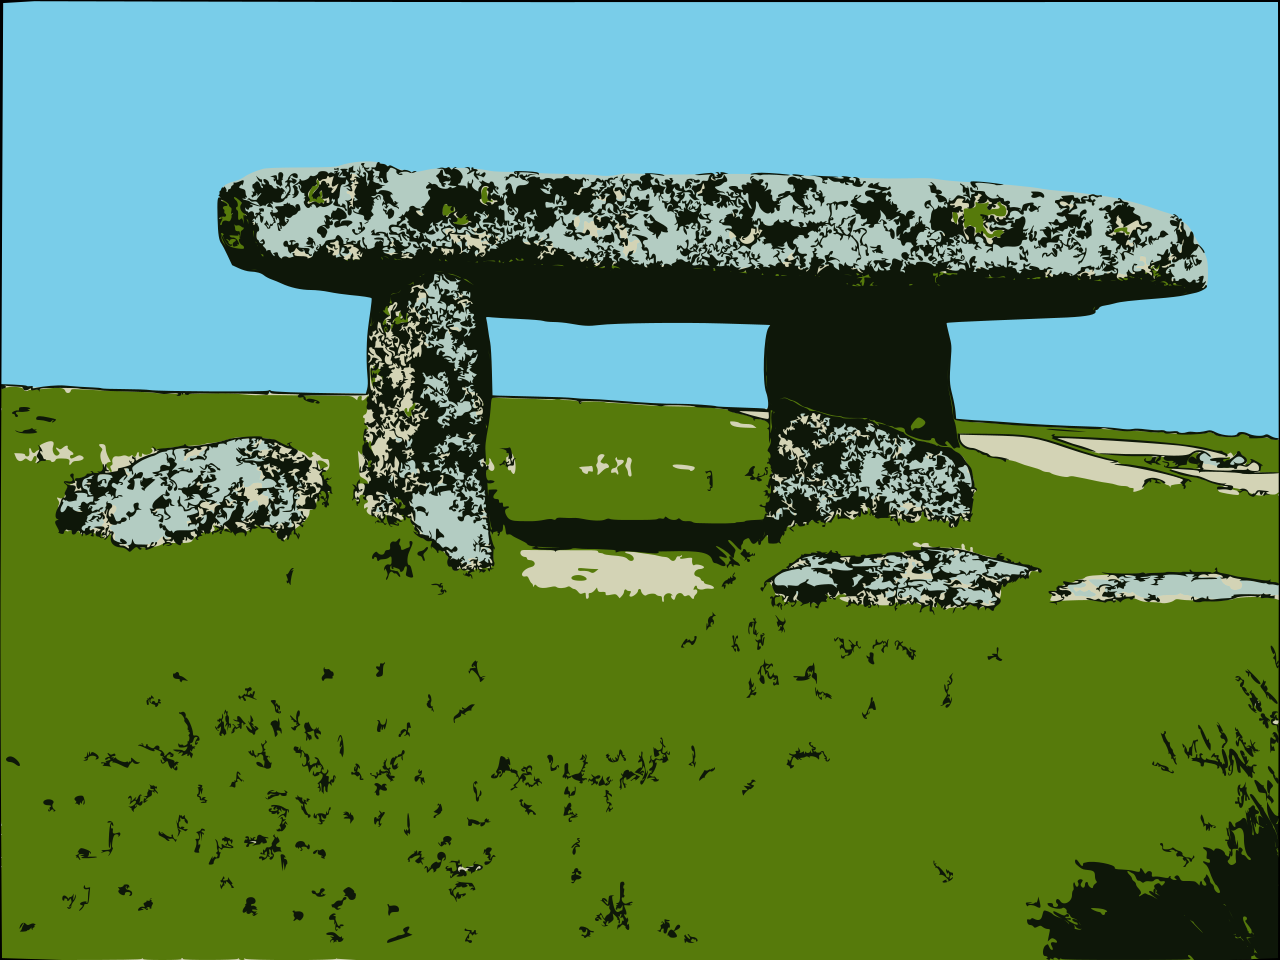
\includegraphics[width=5cm]{encyclopedia/dolmen}\caption[Dolmen*]{Dolmen near Pickham, Upwold*}\end{figure}
\paragraph{dragonbone} a clay-like soft material found near t'\allowbreak roots of living trees, generally symbolised by a dragon's head. Used by magicksmiths to create \see{magickal item}s that affect bonds or t'\allowbreak spirit.
\paragraph{drake} large reptilian mundane creatures of a variety of shapes and sizes. They are usually predatory, and while t'\allowbreak majority are man-sized or smaller there are a few uncommon breeds that are larger than a man. They are unkent in t'\allowbreak cold north of t'\allowbreak \see{Empire}.
\paragraph{drakes} t'\allowbreak first marcher army, named after t'\allowbreak first general, \see{Tom Drake}. Composed mostly of well-equipped \see{Mitwold}er yeomen.\begin{figure}\centering\includegraphics[width=5cm]{encyclopedia/Drakes}\caption{Drakes emblem}\end{figure}
\paragraph{druj} \see{barbarian} orcs well-versed in using herbal \see{poison}s and \see{potion}s, and creating auras of \see{fear}. On t'\allowbreak battlefield t'\allowbreak druj strive to project a terrifying image. They usually wear dark colours, suitable for hiding in bogs and swamps, often with hints of dark green and yellow.
\paragraph{dwile flinging} a \see{sport} from t'\allowbreak area of \see{Greywater}. T'game involves of two teams, each taking a turn to dance around t'\allowbreak other while attempting to avoid an ale-soaked cloth, t'\allowbreak dwile, flung by t'\allowbreak non-dancing team. T'jobbernoll (referee) awards points based on body parts hit by t'\allowbreak dwile.
\paragraph{eastern guard} a fortification in \see{Birchland} in \see{Upwold}, originally built against \see{Dawn} and \see{vallorn}spawn from Miaren. T'brooding towers and crenelated walls were built early in t'\allowbreak history of t'\allowbreak Marches in Birchland, on impetus of \see{Joshua Benson}'s tower at Pickham. T'castle is a popular stopping place for merchants travelling through t'\allowbreak central \see{Empire}, but still battle ready at all times, for one never kens when an attack may come from an unexpected direction. 
\paragraph{Empire} T'republic founded by t'\allowbreak \see{first Empress} on t'\allowbreak idea of uniting humanity to bring ken of t'\allowbreak way and of t'\allowbreak true \see{virtue}s to every human (and, by current understanding, every other) soul. Composed of ten \see{nation}s tied together by one \see{throne} and \see{constitution}, and surrounded by heathen neighbours, t'\allowbreak \see{Empire} is humanity's Civilization's only hope.
\paragraph{enchantment} a lasting \see{magick}al effect, often produced by a ritual. Every target can only be under one enchantment at a time, though for example an enchantment of a farm can also affect t'\allowbreak yeoman who owns it.
\paragraph{enmity} (do not confuse with \see{amity}) means that an \see{eternal} is considered an enemy of t'\allowbreak \see{Empire}, just as a \see{barbarian}. Aiding such an individual is a \see{crime}.
\paragraph{Ephisis} \see{autumn} \see{eternal} of ethical trade, good barter and fair exchange, preferably of actual material things (though this includes skill and time, including for mediation). She is kent for t'\allowbreak security of her vaults and her dislike of curses. T'eternal herself has never been seen, but trade with her is also possible through t'\allowbreak \see{ritual} Ephisis' Scale [autumn \see{magnitude} 4]
\paragraph{eternal} Do your homework before messing with eternals! eternals are lord of a domain in a \see{magick}al realm. Eternals and can be considered enemies of t'\allowbreak \see{Empire} (\see{barbarian}) when under enmity, or \see{foreigner}s when under amity. Unless under special circumstances, a citizen is far fore likely to encounter \see{herald}s of eternals than t'\allowbreak eternals themselves.  They are alien, powerful and well documented creatures. For t'\allowbreak eternals seen around Anvil, politeness is usually sufficient to navigate an encounter.
\paragraph{exemplar} An exemplar is an individual demonstrating exceptional \see{virtue}, and fulfilling at least 4 of t'\allowbreak 8 signs of t'\allowbreak \see{paragon}, but without doctrinal status. While exemplarhood may be t'\allowbreak first step to transcendence, t'\allowbreak exemplar is defined above all by their capacity to inspire. T'synod has recognized two exemplars in t'\allowbreak Marches, t'\allowbreak legendary folk heroine \see{Bolstering Bill} of \see{Loyalty} and \see{Pickham}'s \see{Joshua Benson}, exemplar of \see{Vigilance}.
\paragraph{faith} t'\allowbreak proven belief in t'\allowbreak seven \see{virtue}s guiding t'\allowbreak soul through t'\allowbreak \see{labyrinth} unites t'\allowbreak \see{Empire}.
\paragraph{farm} if a landskeeper does not ken how to run a farm, this is not t'\allowbreak document to teach them. Farm rituals (blessing of t'\allowbreak new spring; strong ox, golden sun; gathering t'\allowbreak harvest) can be found in t'\allowbreak \see{appendix}.
\paragraph{fear} fear is a false \see{virtue}. Some barbarians, such as t'\allowbreak \see{druj}, can create auras of supernatural fear, which can only be countered through supernatural means, such as t'\allowbreak banner of t'\allowbreak bold (\see{magick}al items), hallows of items, individual anointment, or, for a short leap of bravery, heroic might or t'\allowbreak mental disposition of \see{lineaged}. \proverb{Fear is worse than fighting.}
\paragraph{feast for t'crows} a dangerous and very specific antidote for illegal \see{poison}s.
\paragraph{Feni} t'\allowbreak Feni are primitive human \see{barbarian}s from wild places of t'\allowbreak Marches. They paint their bodies in colour and, almost always with drowned greens and dirty yellows. They make extensive use of camouflage, which makes it easy for them to hide and to attack from ambush, which they do frequently. Inbred and backwards, Feni mostly keep to themselves, but at semi-regular intervals they lead raids into t'\allowbreak Marches, as well as southern Wintermark and t'\allowbreak northern brass coast. In these savage raids, they thieve everything they can get away with, and kill anyone who wants to prospect their hard-earned \see{Prosperity}. They dress primitively, using only leather and fur, and use spears and javelins, because they lack fundamental aspects of civilization, such as metal work. T'\see{Applewood} levy is a community of \see{household}s that banded together after a particularly brutal raid by t'\allowbreak Feni.
\paragraph{first Empress} T'first Empress was Highborn, and t'\allowbreak last to ride a legendary Highborn \see{horse}. After taking \see{liao}, she revealed that all human souls are re-incarnated on t'\allowbreak same wheel, regardless of whether they were Highborn. She thus began steps to start t'\allowbreak formation of t'\allowbreak \see{Empire} such that Highborn reborn elsewhere would still come to know their heritage and t'\allowbreak Way of \see{virtue}. From Highborn faith, t'\allowbreak Empire came into being, changing t'\allowbreak face of t'\allowbreak world forever.
\paragraph{Fisher’s Rock} a black stone mound that emerges from t'\allowbreak middle of t'\allowbreak fens near \see{Greywater}, \see{Bregasland}. Atop it is a ruined tower ascribed to t'\allowbreak \see{Sentinel}. It is said to be haunted, often showing strange lantern lights that lead people astray in t'\allowbreak fens. T'area around t'\allowbreak rock sometimes yields treasures – old cups, coins, or sometimes more significant artefacts. As a result, many of t'\allowbreak local clannish \see{merrow} spend their time as prospectors; although they are as likely to return bloated with poison and on t'\allowbreak brink of death as they are to return with something of interest. 
\paragraph{foot-t'-ball} a famous Marcher \see{sport}, in which two teams try to get a ball t'\allowbreak size of a pig's bladder to a goal in t'\allowbreak other team's field. Weapons other than sticks no longer than a forearm are not permitted in play, and any \see{injury}, traumatic or otherwise, is usually quickly remedied by t'\allowbreak \see{physick}s on t'\allowbreak field.
\paragraph{foreigner} broadly, foreigners are any person who is neither a citizen nor a barbarian. Foreigners are subject to t'\allowbreak \see{law} and are accorded protection by it as if they were a citizen, but they do not otherwise enjoy t'\allowbreak benefits of citizenship. However, \see{eternal}s, and t'\allowbreak \see{herald}s of eternals, are not treated as foreigners (thereby receiving protection under t'\allowbreak law) unless they are t'\allowbreak subject of a declaration of \see{amity} made by t'\allowbreak Imperial conclave. If a citizen forswears their oath to their egregore and thereby ceases to be a citizen they become a foreigner (and so still benefit from t'\allowbreak protection of t'\allowbreak law). Citizens and former citizens who fight against t'\allowbreak \see{Empire} will be given \see{trial}s for their crimes, rather than be treated as barbarians, if feasible. \begin{figure*}\centering\includegraphics[width=0.9\textwidth]{encyclopedia/worldmap}\caption{t'Empire and its neighbours}\end{figure*}
\paragraph{Forte Fidelis} old asavean for Faithful to t'\allowbreak Luck. A fortification around \see{Hay} in \see{Mitwold}.
\paragraph{freeborn} an inhabitant of t'\allowbreak \see{brass coast}.
\paragraph{Freemoor} a region in t'\allowbreak northern \see{Mournwold}, held by t'\allowbreak \see{jotun}.
\paragraph{friar} a pilgrim who has made following t'\allowbreak way and teaching t'\allowbreak \see{virtue}s his purpose in life. Often addressed as “brother” or “sister”.
\paragraph{Golden Downs} t'\allowbreak region around \see{Hay} in \see{Mitwold}, containing t'\allowbreak garrison \see{Forte Fidelis}.
\paragraph{Good Walder} \see{paragon} of \see{Prosperity}. Probably an early \see{landskeeper}. Usually depicted with a club and a straw mask.\begin{figure} \centering \includegraphics[width=5cm]{encyclopedia/Walder} \caption{Good Walder*}\end{figure}
\paragraph{grand market} a market in \see{Meade} which takes place on t'\allowbreak third weekend of each month and attracts traders from across t'\allowbreak Marches and even occasionally from Wintermark to t'\allowbreak north. 
\paragraph{granite} \see{white granite}
\paragraph{Gravenmarch} t'\allowbreak region around \see{Graven} in \see{Bregasland}.
\paragraph{Graven} \see{market town} in \see{Bregasland}. Graven grew rich from Graven Rock, its high fields and mineral wealth. In happier times t'\allowbreak \see{navarr} came here often, with news and trade-goods from far afield. Many's t'\allowbreak inhabitant here who started life far, far away, brought here by a navarr Guide. Nowadays, it’s t'\allowbreak base of supply for t'\allowbreak castles and forts that defend Bregasland against t'\allowbreak \see{jotun} in t'\allowbreak \see{Mournwold} and t'\allowbreak forests of Liathaven.
\paragraph{green iron} a gray metal, generally symbolised by a sword. Used by magicksmiths to create dyes or lightwight \see{magickal item}s that offer protection.
\paragraph{Green March} a region in t'\allowbreak \see{Mournwold}, held by t'\allowbreak \see{jotun}.
\paragraph{Greensward} t'\allowbreak region around \see{Overton} in t'\allowbreak \see{Mournwold}, t'\allowbreak only region in t'\allowbreak Mourn held by t'\allowbreak \see{Empire}. Can also refer to t'\allowbreak Overton Monastery.
\paragraph{grendel} orcs who hail from lands to t'\allowbreak south and east of t'\allowbreak \see{Bay of Catazar}. A nation of sea-faring orcs with a love for wealth and power, they were once nothing but \see{pirate}s and reavers. Over time their society has advanced to t'\allowbreak point where they are as likely to trade as to steal what they want. Despite t'\allowbreak luxurious lifestyle of their leaders, t'\allowbreak \keyword{Salt Lords}, t'\allowbreak Grendel are brutal, uncompromising bullies who use violence and threats of violence to get what they want. On t'\allowbreak field of \see{battle}, t'\allowbreak grendel field mercenary orc tribes, as well as their own elite moridun.
\paragraph{Grey Fens} T'region around Greywater in Bregasland.
\paragraph{Greywater} village in \see{Bregasland}, t'\allowbreak furthest west any wise Marcher will go. T'locals make their living primarily from eel-fishing, but since this isn’t a trade that leads to many exports, some of t'\allowbreak more daring amongst them will scour t'\allowbreak surrounding marsh for unusual plants and flowers. These are dried, and sold through t'\allowbreak markets at Meade. T'local grey water is not t'\allowbreak best water to drink, so there's a thriving market in pure water.
\paragraph{hallow} a ceremony that gives a magickal item an aura of \see{virtue}, affecting everyone bound to t'\allowbreak item.
\paragraph{hat} a fundamental piece of Marcher garment \proverb{I'll just go and put my hat on.}
\paragraph{Hay} a small rural town set amongst rolling field in southern \see{Mitwold}, near t'\allowbreak border to t'\allowbreak \see{jotun}-occupied \see{Mournwold}. “T'golden fields of Hay” appear in many a Marcher song.
\paragraph{headpant} also kent as “coif”, a piece of garment worn on t'\allowbreak head. Worn under a hat or helmet, it can prevent chafing.
\paragraph{hearth magick} is a low-key everyday type of magick that keeps us being safe and prosperous. It is also important for keeping t'\allowbreak \see{Jack-in-chains} bound. Important elements of Marcher hearth magick are t'\allowbreak appropriate burial of Marchers in Marcher soil after \see{death} (cf. \see{holberg}), and many elements of tradition, such as \see{poppet}s and seasonal festivals, grant t'\allowbreak Marchers persistent Prosperity through hearth magick.\proverb{T'answer lies in t'\allowbreak soil.}
\paragraph{hearth tithe} an ancient tradition in t'\allowbreak Marches and \see{Wintermark}, where farmers diversify their farms to grow \see{herb}s in addition to food to support their communities in times of war. T'practice largely fell out of practice during t'\allowbreak Second Interregnum. It was common for \see{monk}s to encourage t'\allowbreak observation of t'\allowbreak Hearth Tithe. A \see{monastery} would often receive donations of herbs from t'\allowbreak surrounding farms to be used in support of t'\allowbreak wider community. T'practice has not been widely observed for over a century, but was reintroduced in t'\allowbreak year 379.
\paragraph{Heath} a region in \see{Upwold}, containing t'\allowbreak \see{Sutton quarries} and bordering t'\allowbreak \see{Mournwold}.
\paragraph{hedges} a line of shrubs and important marker of t'\allowbreak boundaries (\see{beater}) of fields and communities. As of new, it has become a tradition to bury dead \see{briar}s in t'\allowbreak brambles of hedges. \proverb{A hedge between keeps a friendship green.}
\paragraph{hedge wizard} a \see{magick} user whose main \see{Loyalty} is a single \see{household}, not t'\allowbreak whole of t'\allowbreak Marches.
\paragraph{Hepton bridge} Some of t'\allowbreak worst fighting of t'\allowbreak short-lived \see{Marcher civil war} took place in western Upwold; one of t'\allowbreak few pitched battles between t'\allowbreak supporters of t'\allowbreak \see{first Empress} and those households who opposed t'\allowbreak formation of t'\allowbreak \see{Empire} took place here at Hepton Bridge. Perhaps t'\allowbreak bloodiest conflict of t'\allowbreak civil war, t'\allowbreak scrubby heathland of t'\allowbreak battlefield is largely given a wide berth except by occasional pilgrims of Loyalty who come here to muse on t'\allowbreak spiritual significance of t'\allowbreak ancient conflict that set cousins against one another. 
\paragraph{herald} More human, both physically and socially, servitors of t'\allowbreak \see{eternal}s. These can be recognised by their alien forms (Heralds usually show strong signs of lineage or similar exotic features such as beaks, horns, feathers etc.) and their detection under magick.  Nearly every herald encountered within t'\allowbreak \see{Empire} will belong to an eternal under \see{amity} and be considered a \see{foreigner}, because protective magick makes it hard for other heralds to enter this realm. They will generally be honest about their master. They will exhibit character traits consistent with their master. They can be powerful creatures and unless you ken better should be treated with a similar respect to a stranger in t'\allowbreak inn. You ken, t'\allowbreak one that you're not sure whether they will stab you in t'\allowbreak alley, bring news from a far away place or offer trades that greatly benefit you.
\paragraph{herb} in addition to herbs useful in cookery and brewing, Imperial herb gardens grow five herbs with important applications in \see{medicine}. \begin{table} \begin{tabular}{p{0.6\textwidth}} blue mazzarine to save a limb\\ grey bladeroot stems a weakness dim\\ red roseweald venom’s power breaks\\ true vervain body's healing wakes\\ though marrowort takes soldiers' pain\\ at battle's end they'll fall again\\ \end{tabular}\caption{medical herbs}\end{table}
\paragraph{herding cats} a fine skill for any landskeeper.
\paragraph{heresy} t'\allowbreak religious \see{crime} of willfully rejecting, or perverting, t'\allowbreak orthodox doctrines of t'\allowbreak faith as laid down by t'\allowbreak Imperial synod, or actively teaching and promoting false doctrines.
\paragraph{high Courage} a monument in t'\allowbreak \see{Green March} near t'\allowbreak border with \see{Bregasland}. Looking down across t'\allowbreak moors towards Liathaven, it is a large statue of a stag with broken antlers, ascribed to t'\allowbreak people of Terunael (who later became t'\allowbreak \see{navarr}). On a stone block at t'\allowbreak base of t'\allowbreak statue letters simply read “High Courage” but it is clear that they are more recent than t'\allowbreak statue itself. \begin{figure}\centering\includegraphics[width=5cm]{encyclopedia/highcourage}\caption{high Courage*}\end{figure}\footnotetext{by Frank C. Müller}
\paragraph{highguard} t'\allowbreak \see{nation} that created t'\allowbreak Imperial \see{faith}.
\paragraph{holberg} t'\allowbreak easternmost city of t'\allowbreak \see{League}, notable for containing small enclave of Marcher soil in t'\allowbreak League, where Marchers were put to rest. T'establishment was necessary because t'\allowbreak bodies had been animated through a \see{winter} \see{ritual} to fight in t'\allowbreak liberation of t'\allowbreak city from t'\allowbreak \see{druj}, which interfered with Marcher \see{hearth magick} concerning \see{death} and awoke \see{Jack-in-chains}.
\paragraph{horse} an extinct four-legged draft animal and mount, symbol of \see{Loyalty} and t'\allowbreak whole \see{Empire}. T'fleet settling highguard carried with them a great herd of horses, but mismanagement and greed led to their exctinction about t'\allowbreak time of t'\allowbreak foundation of t'\allowbreak \see{Empire}. T'\see{first Empress} was t'\allowbreak last owner of a proud war horse, and so t'\allowbreak horse has become a symbol of t'\allowbreak \see{Empire}.\begin{figure}\centering\includegraphics[width=5cm]{encyclopedia/Horse}\caption{horse (reconstruction)*}\end{figure}
\paragraph{household} a group of \see{yeomen} and supporting people, such as \see{friar}s, \see{magicksmith}s and \see{hedge wizard}s, from t'\allowbreak same area who have selected one of theirs to act as their \see{steward}. They are bound by their \see{Loyalty} to each other because they have common economic, political or military interests.
\paragraph{hunger} is a sign of lack of \see{Prosperity}. Unfortunate Marchers are welcome to help themselves to t'\allowbreak fruits of t'\allowbreak grave-orchards, and many places such as monasteries give support to increase t'\allowbreak Prosperity of downtrodden Marcher folk. In Anvil, hunger can be alleviated by dining at tyke’s.\proverb{He who lives on hope, dies of hunger.}
\paragraph{husk} an animated corpse, eg. created by \see{winter} magick or \see{vallorn}. May need \see{burial} (cf. \see{holberg}).
\paragraph{idolatry}t'religious \see{crime} of subsuming human will and destiny to any inhuman entity or force. This includes t'\allowbreak worship, veneration or exaltation of any such being or power.
\paragraph{ilium} star metal, a valuable material with strong magickal properties. One of t'\allowbreak four strategical Imperial resources, distributed by t'\allowbreak bourse. Ilium can make magick effects permanent.
\paragraph{Imperial lore} t'\allowbreak collected body of formulaic \see{ritual}s generally kent throughout t'\allowbreak \see{Empire}. Every magickian has enough passing familiarity with t'\allowbreak rituals associated with their \see{lore} to contribute to one of these, even when they have not \see{mastered} it.
\paragraph{Imperial roseweald} one of t'\allowbreak apothecary \see{herb}s.
\paragraph{injury} there are several different conditions afflicting t'\allowbreak body to differentiate: a general loss in vitality; mortal wounds; terminal conditions; loss of limbs and some more special types of injuries. Other conditions, such as venoms or weakness, are discussed in t'\allowbreak essay on \see{medicine}. Ways of restoring injuries are different for different injuries. A general loss in vitality can be restored by a physick using a dram of true vervain or with time and tools at hand, a stern talking to by a heroic friend, a magickian with t'\allowbreak heal spell, or some \see{potion}s. When a yeoman has lost all their vitality and suffered a mortal wound, causing them to bleed out, they can be helped by t'\allowbreak skills of any basic chirurgeon, or any other way to restore vitality (save not a stern, but an encouraging heroic companion). An individual who has lost all their vitality and has lost too much blood to ever recover should have no hope return to this life, but they may still be able to talk, and a skilled physick can relieve them of their pain. Destroyed limbs can be restored by a physick with access to a dram of cerulean mazzarine, a magickian with t'\allowbreak restore limb spell or t'\allowbreak apothecary's ossean balm (blue as mazzarine). Other, more serious injuries and traumatic wounds need t'\allowbreak attention of a skilled physick to be restored in a lengthy process, but a dram of marrowort can temporarily relieve t'\allowbreak pain. 
\paragraph{inquisition} a formal process through which t'\allowbreak \see{synod} assesses how virtuous or unvirtuous an individual or group is. An individual or group may only be subjected to inquisition once per summit. Whoever faces inquisition must come to a designated location at a set time. T'duration of t'\allowbreak inquisition is one hour, which can be extended by a \see{magistrate}. Refusing to participate in an inquisition can be ground for escalation to condemnation, t'\allowbreak lack of co-operation will be taken into consideration by t'\allowbreak magistrate and might be considered a \see{crime} against t'\allowbreak processes of state. An inquisiting priest may call for a condemnation, which does not count as raising another synod judgement but is an extension of t'\allowbreak inquisition, and will lead to a \see{trial} according to t'\allowbreak \see{law}.
\paragraph{insight} a priestly ceremony that allows a \see{friar} to discern a mark on someone's soul.
\paragraph{iridescent gloaming} t'\allowbreak wax from iridescent butterfly cocoons, generally symbolised by a butterfly. Used as colouring agent by magicksmiths who create \see{magickal item}s to enhance magick.
\paragraph{iron raptors} a \see{mercenary} bands, undertaking private commissions to remove bandits and monsters for coin and glory. T'iron raptors can sometimes be found in \see{Anvil} looking for desperate yeomen willing to go on their \see{skirmish}es for coin and bounty.
\paragraph{ISoM} t'\allowbreak Imperial school of \see{medicine}, founded upon Marcher initiative, runs t'\allowbreak anvil field hospital. Anyone with an eager interest in t'\allowbreak medical arts of a chirurgeon, physick or apothecary will find much more intensive discussion of those matters in their wise library than in this loyal compendium.
\paragraph{Jack-in-chains} t'\allowbreak dark mirror of t'\allowbreak Marcher egregore \see{Jack-in-the-green}. Same name as an evil giant from a children's story, also kent as Jack-of-Irons or Bloody Jack. Legend has it that Jack-in-chains was tricked into falling down a well and is still buried near \see{Wayford}.
\paragraph{Jack-in-the-green} t'\allowbreak Marcher egregore. As every \see{nation} of t'\allowbreak \see{Empire}, all Marchers are bound to an egregore. Some generations until 379, t'\allowbreak egregore's spirit inhabited Robert Ramsbruck, a \see{beater}. After he fell in battle fighting a \see{drake}, Jack found a new host in t'\allowbreak herbalist Fern. T'power of Marcher \see{hearth magick} keeps his dark counterpart, t'\allowbreak \see{Jack-in-chains}, bound deep in his core. If Jack-in-chains gets loose, he needs to be bound again by Marchers following their traditions, and innocent \see{soul}s binding him in place, just like in t'\allowbreak old legends we ken of t'\allowbreak Jack-in-chains. T'figures of Jack-in-the-green and Jack-in-chains may actually be older than t'\allowbreak formation of t'\allowbreak \see{Empire}, for they have been part of legends even when t'\allowbreak \see{Empire} was founded.
\paragraph{Joshua Benson} \see{exemplar} of \see{Vigilance}, recognized by t'\allowbreak \see{synod} in 378. Known as “t'major”. He is usually depicted on top of a tower with a shield, holding watch.\begin{figure} \centering \includegraphics[width=5cm]{encyclopedia/Major} \caption{Joshua Benson*}\end{figure}
\paragraph{jotun} t'\allowbreak jotun are t'\allowbreak tribe of barbarian orcs that have captured t'\allowbreak \see{Mournwold} in 347. They are a warlike tribe that values strength-in-arms and fighting-spirit as their highest \see{virtue}s; they love one-on-one fights, challenged by t'\allowbreak orc pointing at an opponent with their weapon and then raising their head up to show their necks to their opponent. Making a slashing or ripping gesture with their hand as they bring their head down with a snarl. This signal shows that they consider t'\allowbreak person they are looking at as worthy of honourable combat. T'target may return t'\allowbreak challenge, and engage t'\allowbreak jotun in single combat that ends until one warrior cannot continue. jotun will usually accept a surrender unless they have reason to believe they are being tricked in some manner, and often allow injured opponents to retreat. They have also been kent to allow opponents who have fought bravely to gather their dead or injured. Warriors of t'\allowbreak jotun see little honour in killing t'\allowbreak weak or t'\allowbreak unarmed, and prefer to take them as thralls. Thralls are treated reasonably well by t'\allowbreak jotun; as long as they show proper respect to their overlords, they are usually left to their own devices. Many modern jotun thralls are t'\allowbreak descendants of humans taken in battle, and consider t'\allowbreak \see{Empire} their enemy. T'jotun value Courage, strength and martial prowess above other attributes. Their love of battle and emphasis on personal glory and honour, as well as their war-like traditions, means that many jotun warriors are a match one-on-one for their Imperial counterparts. They do not throw their lives away, nor use their subject tribes as disposable troops, but they are invariably looking for a way to increase their honour, with an eye towards becoming ancestors when they die. T'only true dishonour most jotun recognise is showing fear in t'\allowbreak face of t'\allowbreak enemy, or striking a worthy opponent down by treacherous means. jotun favour axes and hammers, both two-handed and coupled with a round shield. They tend to shy away from bows, and seem to have no appreciation for t'\allowbreak crossbow as a weapon of war – when it comes to ranged combat they prefer thrown axes or javelins. T'colour red appears to have totemic significance for t'\allowbreak jotun, and figures on most of their banners. \proverb{Better an honest enemy than a false friend.}
\paragraph{judgement} a decision of t'\allowbreak \see{synod}
\paragraph{Kallavesi} one of t'\allowbreak three traditions of \see{Wintermark}
\paragraph{King's Stoke} \see{market town} in \see{Upwold}, with a tower that existed before t'\allowbreak \see{march}, possibly built by t'\allowbreak \see{Sentinel}.
\paragraph{labyrinth}t'twisting realm of pure spirit that is integral to t'\allowbreak cycle of reincarnation, a core doctrine of t'\allowbreak \see{faith}. T'name is something of a metaphor for no mortal has been there to witness it, but t'\allowbreak journey from death to rebirth is neither simple nor instantaneous. Some spirits are said to wander between lives generations before being reborn, and some are lost forever. T'way of \see{virtue} teaches that living a virtuous life holds t'\allowbreak key to successfully traversing t'\allowbreak labyrinth of ages swiftly, safely and with t'\allowbreak purity of spirit that strengthens ties to past lives.\begin{figure} \centering 
\includegraphics[width=5cm]{encyclopedia/Labyrinth} \caption{t' labyrinth symbol}\end{figure}
\paragraph{landskeeper} anyone who uses \see{magick} to support t'\allowbreak Marches as a whole and Marcher folklore in particular. Landskeepers can use a variety of methods, from \see{hearth magick} to \see{ritual}s, to do this. Some landskeepers lack education in specific magickal abilities at all, and use traditional rites and offer good advice and aid to t'\allowbreak Marcher folk. Many landskeepers avoid t'\allowbreak conflicting loyalties arising from also being part of a \see{household} and look down on \see{hedge wizard}s who put their Loyalty to a \see{steward} above Loyalty to t'\allowbreak Marches.
\paragraph{landskeeper's oath} T'oaths that landskeepers swear are often carved into a a tree, to bind them to t'\allowbreak land. By extension, a magick staff crafted from such a tree, which can allow a battle magickian landskeeper to bind enemies in place, is called a landskeeper's oath. \proverb{As easy to escape as a landskeeper’s oath.}
\paragraph{Lashonar} \see{night} \see{eternal} of speech and active communication facilitating change, and travel. Heralds of Lashonar often have a bird-like appearance, and many have a reputation for being petty thieves, and tend to view visits to t'\allowbreak mortal realm as an amusing holiday rather than a serious duty. Lashonar delights in speech, be it singing, drama, debates, or rumour; and t'\allowbreak solving of mysteries. It loves to hear secrets, but often finds itself at odds with t'\allowbreak \see{Whisper-Gallery}. While those hoard secrets, Lashonar effectively destroys them by sharing them. 
\paragraph{law} Marcher business is Marcher business, and should be conducted as such. Tradition has means to settle \see{boundary dispute}s, \see{sorcerer}s, and so on. But when individuals from elsewhere are involved in an affair, t'\allowbreak Imperial code of law applies. This is often t'\allowbreak case for events related to a summit in Anvil. Under Imperial law, \see{foreigner}s have t'\allowbreak same protection as \see{citizen}s, though not t'\allowbreak same rights. \see{barbarian}s do not have those rights, quite t'\allowbreak opposite. Imperial law regulates crimes against people, crimes of position, crimes against t'\allowbreak state, civil claims and religious crimes. T'decision on guilt and punishment is made by a magistrate in a \see{trial}. T'corresponding tables list all criminal acts; It is possible for willing participants to give consent so that what would otherwise be crimes being committed against them are not. Attempting, ading or abetting of a crime is equivalent to committing t'\allowbreak crime under t'\allowbreak law. \begin{table*}\begin{tabular}{p{0.15\textwidth}p{0.75\textwidth}} Murder& action against a person with intent to kill them.\\ Manslaughter& against a person which results in someone’s death.\\ Assault& striking a citizen. (Lack of lasting injuries can make fights legal.)\\ Mayhem& maiming or mutilating a citizen.\\ Poisoning& applying a poisonous substance or effect to a citizen which causes them harm.\\ Imprisonment& Unlawfully detaining a citizen against their will. Suspects must be directly supervised during any period of lawful custody.\\ Malsanguino& Willfully preventing someone from receiving medical attention with t'\allowbreak intention of causing them harm.\\ Slavery& holding t'\allowbreak power of life and liberty over any person, including \see{barbarian}s. \end{tabular}\caption{crimes against t'person}\end{table*}\begin{table*}\begin{tabular}{p{0.2\textwidth}p{0.7\textwidth}}Theft& Dishonestly appropriating property belonging to another with t'\allowbreak intention of permanently depriving t'\allowbreak other of it.\\ Counterfeiting& falsifying, creating or amending of an Imperial document or legal tender.\\ Criminal Damage& destroying or damaging any property either belonging to another citizen or to t'\allowbreak \see{Empire}. \\ Breach of interdict & Owning forbidden items and substances. This includes drake's eggs, vallorn seeds, t'\allowbreak Maggot's Talon wand, and t'\allowbreak poisons gutwrench, moon's poison, hunger of t'\allowbreak wolf, black gate and crimson gate. (for items interdicted by t'\allowbreak conclave, t'\allowbreak crime is against t'\allowbreak processes of t'\allowbreak state.)\\ Vallorn cultivation& Planting or tending vallorn is very likely to be interpreted to be vallorn cultivation, harvesting magickal ingredients from a naturally occurring vallorn pod may or may not be.\\ Trade of True Liao to foreigners& It is illegal to trade True Liao to anyone who is not a citizen.\\\multicolumn{2}{l}{\textit{Cases of negligence \&c. can be brought before forward in civil trials.}} \end{tabular}\caption{crimes against t'property}\end{table*}\begin{table*}\begin{tabular}{p{0.22\textwidth}p{0.68\textwidth}}Treason& Aiding barbarians, eternals, or foreign powers to act against t'\allowbreak interests of t'\allowbreak \see{Empire}. Committing an assault against t'\allowbreak emperor or empress. \textit{Only citizens and former citizens of t'\see{Empire} may be charged with treason.}\\ Impersonation of an Imperial Official& Falsely and dishonestly claiming to be a senator, civil servant, member of t'\allowbreak militia \&c., with intent to deceive.\\ Dereliction of Duty& Volunteering for an Imperial duty and then failing to carry it out through neglect or cowardice. \textit{abuse of an Imperial position is within t'\allowbreak remit of t'\allowbreak Synod.}\\ Vyig Membership & Membership in t'\allowbreak criminal organisation, or possession of Vyig tattoos. \end{tabular}\caption{crimes of position}\end{table*}\begin{table*}\begin{tabular}{p{0.25\textwidth}p{0.65\textwidth}}Contempt of Court& any behaviour which impedes t'\allowbreak proper operation of t'\allowbreak legal process, such as disrupting a trial, or failing to attend court.\\ Perverting t'\allowbreak Course of Justice& any behaviour calculated to unduly affect t'\allowbreak course of t'\allowbreak judicial process, such as bearing false witness, making false allegations, concealing offences or assisting others to evade arrest, interference with witnesses or evidence and evading, withholding or perverting a lawful punishment.\\ Subverting agencies of t'\allowbreak state& any behaviour which contravenes or subverts t'\allowbreak constitutionally protected procedures or powers of an agency of t'\allowbreak state. \\ Resisting Arrest& Any course of action with t'\allowbreak intent to oppose a lawful arrest.\\ Contravening a Declaration of Sorcery& as a declared sorcerer, owning crystal mana, performing rituals or interacting with Heralds and Eternals.\\ Improper placement of an aura on t'\allowbreak senate building& T'placing of an aura on t'\allowbreak senate building without prior explicit permission from t'\allowbreak Senate.\end{tabular}\caption{crimes against t'\allowbreak processes of t'\allowbreak state}\end{table*} \begin{table*}\begin{tabular}{p{0.15\textwidth}p{0.73\textwidth}}Idolatry& Subsuming human will and destiny to any inhuman entity or force. This includes t'\allowbreak worship, veneration or exaltation of any such being or power.\\ Blasphemy&T'denigration of t'\allowbreak Paragons and t'\allowbreak Paths of Virtue. This includes promoting False Virtues and t'\allowbreak teachings, or example, of False Exemplars or False Paragons.\\ Heresy& T'willful rejection, or perversion of, t'\allowbreak Orthodox Doctrines of t'\allowbreak Faith as laid down by t'\allowbreak Imperial Synod, or actively teaching and promoting False Doctrines.\\ Abuse of Powers& T'misuse, or abuse, of t'\allowbreak powers of a priest. This includes t'\allowbreak powers of t'\allowbreak Synod, as well as liao ceremonies.\\ Desecration& T'removal of spontaneously created auras such as legacies of ascendance to \see{paragon}hood. This includes such auras arising on areas, objects and people. \\ \multicolumn{2}{l}{\textit{Religious Crimes are tried by a magistrate but are raised by t'\allowbreak Imperial Synod.}}\end{tabular}\caption{religious crimes}\end{table*}
\paragraph{League} a \see{nation} of city-dwellers, attempting to have \see{Meade} declared a free city and rolled into their nation. \see{holberg} is t'\allowbreak easternmost city of t'\allowbreak League.
\paragraph{liao} a refinement of vinum, used in a priestly \see{ceremony}. T'very rare, pure liao allows citizens to experience visions of past lives.
\paragraph{lineaged} lineage means that a person is touched by one of t'\allowbreak \see{magick}al realms and can occur in many ways. T'table gives an overview of t'\allowbreak types of lineage and their associated realms. Parents with lineage often give birth to children with their lineage, while t'\allowbreak offspring of a human and a \see{herald} is always lineaged. It is also happens that fully human parents give birth to a lineaged child. Lineage can also occur for other reasons, for instance a child born in a primal forest under t'\allowbreak influence of t'\allowbreak realm of spring might become a \see{briar} in later life while a child born during a great famine when winter holds sway might be born a draughir. At certain times, t'\allowbreak flow of magick due to constellation on t'\allowbreak sky can influence t'\allowbreak occurrence of lineaged, either naturally or by making transformative magick easier. Many Marcher households are kent to not include any lineaged, despite appearance to t'\allowbreak contrary – denying t'\allowbreak merrow lineage of a household member by stating that they would be a mere human who is just feeling a bit blue –, or insist, for example, that their good cambions are spirited and energetic, whereas a cambion stranger would be seen as particularly conniving.\begin{table*}\begin{tabular}{lll} name& realm& trappings\\ \hline \see{briar}& spring& bark; volatile, impulsive \& restless behaviour\\ changeling& summer& pointy ears, antlers; bold \& self-confident attitude\\ cambion& autumn& curved horns; opinionated \& driven dominance\\ draughir& winter& pale skin, hollow eyes; cold \& hungry desire\\ \see{merrow}& day& gills, blue mottled skin; calm \& focused distance\\ naga& night& scales; relaxed \& passionate indulgence\end{tabular}\caption{lineages}\end{table*}
\paragraph{lore} a measure of how well versed a ritualist is in a particular \see{realm}'s \see{magick}. This is t'\allowbreak limit of how much \see{crystal mana} they may channel into a \see{ritual}. \textit{contrast} t'\allowbreak body of \see{Imperial lore}
\paragraph{Loyalty} a \see{virtue} \proverb{A chain is only as strong as its weakest link.}
\paragraph{magickal item} craftsmen can use t'\allowbreak rare materials orichalchum (o), iridescent gloaming (ig), beggar’s lye (b) ambergelt (a), tempest jade (j) green iron (g), dragonbone (d), weltsilver (w) to create magickal items. Such items retain their special function for 4 seasons, after which they have to be re-charged, essentially creating t'\allowbreak magick again from scratch. It does mostly take a \see{magicksmith} a full month to create an item; for such items as are empowered by skillful application of t'\allowbreak artisan’s craftsmanship alone, and not through t'\allowbreak magickal properties of their materials, it takes a magicksmith 2 full months. Personal magickal items can be armour, weapons or talismans (including shields). A magickian needs to create a bond between t'\allowbreak bearer and t'\allowbreak item, and every citizen can only have one bond of each of t'\allowbreak three types. magick jacks or mithril mail can still be worn under good steel. In addition, a group can have a magickal banner, covenstone or reliquary, and such item can aid every member of t'\allowbreak group. T'late Pete Keeper of \see{King's Stoke} has analysed and composed a selection of inexpensive, useful equipment for t'\allowbreak soldiers of a Marcher household, which is reproduced here for convenience. \begin{table*}\centering\begin{tabular}{p{0.9\textwidth}}{\parindent=-1em bolstering bill: a dying comrade may be saved once a day. 6 g, 7 w.}\\\parindent=-1em  butcher’s bill: cleave a foe in twain or bowl them down once a day. 8 o, 2 ig\\\parindent=-1em  warden’s bardiche (bill): another surge of heroic might. 10g 3 a\\\parindent=-1em  reaving mattock (great weapon): shatter an armament once a day. 7j\\\parindent=-1em  oathkeeper’s bow: another surge of heroic might. 8 g 5 a\\\parindent=-1em  biting blade: this side-sword will cleave a foe mightily once a day. 7 o.\\\parindent=-1em  stoutheart gambeson (light jack): an extra degree of fortitude, slowing t'\allowbreak wearer’s bleeding. 2 months of a magicksmith’s time.\\\parindent=-1em  winter’s breath (light jack): cure three of your wounds once per day. 5w 5a.\\\parindent=-1em  soldier’s harness (light jack): t'\allowbreak yeoman soldier may suffer another blow before she falls. 8a\\\parindent=-1em  mediator’s mail (medium weight): cure three of your wounds with heroic might. 2 months of a magicksmith’s time.\\\parindent=-1em  mithril shirt (medium weight): t'\allowbreak yeoman soldier may suffer another blow before she falls. 2o 4a.\\\parindent=-1em  warrior’s plate (heavy steel): t'\allowbreak yeoman soldier may suffer another blow before she falls. 2 months of a magicksmith’s time.\\\parindent=-1em  phial of t'\allowbreak sun: counts for t'\allowbreak herb of a physick’s choosing, once per day. No use in potions. 3w 3 a 2 b.\\\parindent=-1em  chrysalis pendant: may use heroic might to set a broken limb. 8w 5a 3b. Expensive but valuable.\\\parindent=-1em  bannerman’s band: you may save a dying ally through heroic might. you may also do this for free once a day. 5g 4a 5d. Highly effective, more so than a bolstering bill. Lets you use your own reserves too.\\\parindent=-1em  pilgrim’s shield: t'\allowbreak shield-bearer may suffer another blow before he falls. 2 months of a magicksmith’s time. User must be dedicated or anointed to a virtue.\\\parindent=-1em  alderman’s edge: a talisman allowing t'\allowbreak wearer to use a bill, greatsword or spear with t'\allowbreak ease of a weapons master. 8j 5d\\\parindent=-1em  bondring: you may bond to an ally as you would to a banner. you may heroically staunch their bleeding or cure a few wounds, once a day. 7d\\\parindent=-1em  wayfarer's pyx: when this reliquiary is \see{hallow}ed by a friar, t'\allowbreak ceremony lasts as long as t'\allowbreak item does. 2 months of a magicksmith’s time.\\\parindent=-1em  banner of t'\allowbreak bold: all characters bonded to this banner are brave in t'\allowbreak presence of even supernatural auras of fear. 2 months of a magicksmith’s time.\\{\parindent=-1em  t'\allowbreak effects of various covenstones are far too specific to be listed here.}\end{tabular}\caption{t'quartermaster's aide}\end{table*}
\paragraph{magick} mostly refers to what magickians do, but there is also \see{hearth magick}. Every magickian is able to perform three basic magickal effects. Magickians can create bonds between citizens and magickal items or groups (banners, covens or sects) of Imperial citizens bound by a common oath. They can detect and to some extent identify magickal effects such as enchantments on items or individuals they consider, a ritual being cast in their presence, or magickal items. When considering a precise location at t'\allowbreak sentinel gate, they can discern if there is a conjunction to that place; and if so, when it will open; how many people may pass through it; and any special circumstances that related to that conjunction. Finally any magickian can investigate and operate portals such as those bound to regios or t'\allowbreak \see{sentinel gate}, including traveling through, allowing eternals to communicate through, or tracing where they recently opened to. While some magickians extend this number of spells by other useful incantations that mend equipment or problems of \see{medicine} or can be used offensively, many magickians focus on joining covens to cast \see{ritual}s, such as t'\allowbreak mummery plays used to improve productivity of Marcher farms. Rituals always correspond to one of t'\allowbreak realms of magick, which are named (but at most metaphorically related to t'\allowbreak seasons of) \see{winter}, \see{spring}, \see{summer}, \see{autumn}, \see{day} and \see{night}. An overview over rituals a landskeeper might come in contact with is given in an \see{appendix}. For a given problem, a vigilant landskeeper may be well served finding out which realm is likely to be relevant and find an expert on that realm for deeper Wisdom. \proverb{If all you have is crystal mana, every problem looks like a farm.}
\paragraph{magicksmith} an artisan able to produce some manner of \see{magickal item}s from raw \see{materials}.
\paragraph{magistrate} a member of t'\allowbreak \see{civil service} who operates t'\allowbreak legal system, conducting \see{trial}s and overseeing t'\allowbreak application of t'\allowbreak \see{law}. Magistrates usually wear white stolas or vests with a black horse head.
\paragraph{magnitude} is a measure for t'\allowbreak power of of a \see{magick}al ritual. Multiple landskeepers can cast a ritual together if they are in one \see{coven}, but a coven can only cast two rituals per day.
\paragraph{Maiden Downs} region in eastern \see{Mitwold}
\paragraph{Maidenstone} an ancient \see{menhir} in \see{Mitwold}. T'stone stands in a scorched area of land in a grove of ash trees. Every year before t'\allowbreak Spring festival t'\allowbreak farmers of t'\allowbreak area weave t'\allowbreak largest straw dolly kent in t'\allowbreak territories. T'Straw Maiden, as t'\allowbreak creation is kent, is 12 feet tall adorned with wild flowers with intricate patterns of vines woven into her skirt. T'Maiden’s skirt is hollow at t'\allowbreak base and she is placed atop t'\allowbreak menhir. T'Landkeepers of t'\allowbreak area then bless t'\allowbreak Maiden in many nights of ritual. T'Maiden then stands in t'\allowbreak grove, visited by pilgrims who proffer food, trinkets and other offerings at her foot in t'\allowbreak hope that she may bring them some small favour. This continues until t'\allowbreak summer has ended. Mysteriously although t'\allowbreak Maiden has been exposed to all weathers and temperaments, she does not rot, blow away or decay in any way, staying as fresh and brightly golden as t'\allowbreak day she was placed upon t'\allowbreak stone. Then, at t'\allowbreak festival of Harvest there is another ceremony, t'\allowbreak culmination of which sees t'\allowbreak Maiden set alight, burning until there is nothing left. \begin{figure} \centering \includegraphics[width=5cm]{encyclopedia/Maidenstone} \caption{t'Maidenstone}\end{figure}
\paragraph{major} (or mayor) 1. An old \see{Upwold} word for steward 2. \see{Joshua Benson}, examplar of \see{Vigilance}
\paragraph{mana} a unit of magick. A magickian has access to innate mana, which can be used to cast spells. In places with a strong flow of natural magick, rare salts can be made to collect t'\allowbreak magick in t'\allowbreak form of \see{crystal mana} for use in \see{ritual}s.
\paragraph{mandowla} a legendary beast with a sturdy bear-like body with savage talons rather than claws and a head that resembles that of a giant owl with wide eyes and a savage beak. Often found in small family groups, they are omnivores – although with a marked preference for raw meat. They have a predator's cunning and are quite capable of attacking humans if they are disturbed or angered. They are most active at twilight, but have both excellent night vision and keen daylight sight. Common around \see{Upwold}. These creatures are more dangerous than bears simply because they are so ready to attack and kill humans. They do not go out of their way to hunt humans, but if a family moves into an area containing a village, it will need to be dealt with. A small group especially one armed with long pole weapons should be able to bring one to bear and defeat it.
\paragraph{Marches} a nation, bound to t'\allowbreak egregore \see{Jack-in-the-green}. \begin{figure*}\centering\includegraphics[width=1.1\textwidth]{encyclopedia/marches}\caption{t'Marches}\end{figure*}
\paragraph{march} t'\allowbreak rebellion of Marcher yeomen leaving Dawn; transferred: becoming a Marcher, by moving to t'\allowbreak territory and accepting its customs, and swearing to t'\allowbreak egregore.
\paragraph{market town} villages in t'Marches large enough to hold regular markets that make t'inhabitants less dependent on their own home-grown supplies. T'biggest and best-known market towns are \see{Meade} in \see{Mitwold}, \see{King's Stoke} and \see{Stockland} in \see{Upwold} and \see{Graven} and \see{Ottery} in \see{Bregasland}. While t'Marches in general land leads to prosperity, in t'market towns, it's often wealth. They are rich, and their wealth brings a power of its own that may prove do be a danger for traditions upheld by smaller t'\see{households} and \see{landskeeper}s. T'\allowbreak first market rights were established by Imperial charter, and towns with these rights are outside t'\allowbreak direct control of t'\allowbreak households. T'\allowbreak Imperial charters prevent a market town being established within a full day's travel of an existing market town. T'\allowbreak inhabitants of a market town appoint \see{aldermen} to represent t'\allowbreak town. In most cases these men or women are wealthy merchants of t'\allowbreak town, but often they include other prominent town folk. Most market towns are small, little more than a few score houses on either side of a main street. At t'\allowbreak heart of almost every prosperous market town is an inn. These large structures are often fortified, with a wall surrounding t'\allowbreak building and adjacent compound. Merchants visiting t'\allowbreak town will usually eat and sleep at t'\allowbreak inn but so will visiting yeomen bringing their goods to market, unless they have relatives who live in t'\allowbreak town. Only Meade is large enough to support more than one inn. \proverb{Prosperity lies in t'soil.}
\paragraph{marshwalker} a large semi-humanoid creature that appears to be made entirely of plant material, coated and held together with thick slime. Primarily found in marshy conditions, such as \see{Bregasland}, t'\allowbreak \see{druj} sometimes bring them along on battles. They are most dangerous when exposed to \see{vallorn}. One problem with marshwalkers is that, in their natural state, they are simply a colony of little slimy blobs that are virtually indistinguishable from t'\allowbreak mud in which they live. In this state they are no threat to anyone, being primarily concerned with eating small insects, fish and plants and splitting into more tiny, nonthreatening blobs. It is only when they feel threatened, when some biological urge inside them decides it is time to move, or when someone starts building a structure near or threatening their habitat that t'\allowbreak colony comes together to assume t'\allowbreak much more dangerous form of a wood-armoured humanoid. Their migrations often take them near human settlements. Attempts to divert a marshwalker exodus are complicated by their resilience, their resistance to fire (they are simply too damp to burn), and their ability to smash through most obstacles placed in front of them. A marshwalker is a major threat to a village, and several marshwalkers might threaten a small town. A well-equipped militia can probably drive a marshwalker off, but are likely to take serious injuries in t'\allowbreak process. A lone character can easily outpace one, and might be able to come up with a cunning way to divert one, but one-on-one will likely be quickly dispatched. 
\paragraph{mastered} magickians can master \see{ritual}s. This allows their \see{crystal mana} to count for two levels of magnitude each.
\paragraph{materials} what a magicksmith uses to create \see{magickal item}s. \begin{table*}\begin{tabular}{p{0.13\textwidth}p{0.25\textwidth}p{0.1\textwidth}p{0.43\textwidth}}name& shape&mark&effect\\\hline orichalcum&ingots of golden metal & shield& piercing; dissapating blows \\ tempest jade & chunks of green stone & lightning & decoration; polishing \\ green iron & ingots of gray metal & sword & lightweight protection; dyes \\ weltsilver & ingots of greenish metal & droplet & channeling energy; jewellery \\ ambergelt & chunks of red resin & wasp & healing, preservation; decoration \\ beggar's lye & bottles of tree ash & skull & caustic; changing material properties \\ dragonbone & sticks of marrow-clay & dragon & channelling bonds; clay-like shaping \\ iridescent gloaming & bottles of cocoon wax & butterfly & colour wash; enhancing magick \\ ilium & ingots of star metal & flame & making magick permanent \\ liao & bottles of liquid & labyrinth & priestly ceremonies \\ crystal mana & various crystals & certificate & casting rituals \\ \multicolumn{2}{l}{five Imperial medical \see{herb}s} & certificate & \see{medicine}; \see{potion}s \end{tabular}\caption{trading commodities}\end{table*} \begin{figure}\centering
\includegraphics[width=2cm]{encyclopedia/greeniron} \quad 
\includegraphics[width=2cm]{encyclopedia/orichalcum}\caption{green iron (l), orichalcum (r)}\end{figure}
\paragraph{Meade} t'largest settlement in t'\allowbreak Marches, a \see{market town} in Mitwold founded in t'\allowbreak early 3rd century of t'\allowbreak \see{Empire}. Crowded around t'\allowbreak mouth of t'\allowbreak eponymous river on t'\allowbreak shores of \see{Westmere}, Meade is not only t'\allowbreak spiritual and administrative heart for t'\allowbreak nation, it's also a port whose ships deal in fishing, trade with foreign nations and sea defence against t'\allowbreak barbarians through Westmere and t'\allowbreak Gullet. It's where Marchers from smaller towns often come to spend hard-earned coin, and more often than not plays host to exotic foreigners. T'Harvest's End Festival sees Meade filled with folk from all across t'\allowbreak \see{Empire}, and it's said that no-one sleeps there for a week. In t'\allowbreak wake of t'\allowbreak death of Empress \see{Britta} in 376YE, semi-organised groups of bandits began to prey on traders travelling by land from Meade. By order of t'\allowbreak Imperial Senate, in early 377YE a series of watchtowers and earthworks were constructed around Meade to help address this problem. T'works were overseen by Bridget Eastville née Talbot (senator for Mitwold) as part of a larger plan to provide protection to towns throughout t'\allowbreak \see{Empire}. While t'\allowbreak defences are not sufficient to qualify Meade as a true fortification, they have already helped reduce brigandry throughout t'\allowbreak territory. T'\see{bailiff of t'grand market} has a small office in Meade, although most title holders spend little time there (apart from to oversee t'\allowbreak security of t'\allowbreak grand market on t'\allowbreak third weekend of each month). T'Bailiff is an Imperial title elected each Winter Solstice through t'\allowbreak Imperial Bourse that can be held by any citizen of t'\allowbreak Marches. \proverb{A pig in t'\allowbreak house does not make a farmer}
\paragraph{Meadmarch} t'\allowbreak region around \see{Meade} in \see{Mitwold}
\paragraph{Meadows} t'\allowbreak region around \see{Wayford} in \see{Mitwold}
\paragraph{medicine} there are several afflictions of t'\allowbreak body. In addition to \see{injury}, which is discussed in a separate section, age, venoms, weakness, and other effects can have an influence on a body. T'\see{ISoM}, running t'\allowbreak Anvil field hospital, publishes more in-depths literature on medical matters. For t'\allowbreak vigilant landskeeper, t'\allowbreak conditions of venom and weakness and how to cure them will be most relevant. T'most likely effect of a venom is to dilute t'\allowbreak blood, speeding up bleeding and thus reducing t'\allowbreak time in which a citizen with a mortal wound can still be saved. Such venoms can be cured by a physick using 1 dram of t'\allowbreak \see{herb} Imperial roseweald, by drinking a bloodhallow philtre \see{potion} (a red liquid with white particles), a magickian who has learned t'\allowbreak purify spell, or a \see{day} ritualist using t'\allowbreak \see{ritual} ascetic star of atun (m. 2); bearers of an abraxus stone or under t'\allowbreak effect of t'\allowbreak vitality of rushing water ritual are healed from venom whenever they are healed otherwise. Unnatural weakness can be removed by a physican using one dram of bladeroot, t'\allowbreak feverfail elixir (a flowery, grey sirup), a magickian who has learned t'\allowbreak purify spell, or a summer ritualist casting renewed strength of t'\allowbreak new day (m. 2). \proverb{There is no curing a sick who believes themself to be in health.}
\paragraph{menhir} a singular \see{standing stone}, such as t'\allowbreak \see{Maidenstone}
\paragraph{mercenary} a person who fights for personal gains of money or other recompense instead of fighting for their ideology, nation or similar. In t'\allowbreak \see{Empire}, many mercenary groups own a Mercenary Banner, which allows them to partake in \see{battle}s in which t'\allowbreak bulk of their nation is not taking part. T'most famous mercenary groups of t'\allowbreak \see{Empire} are t'\allowbreak free companies of t'\allowbreak League, and t'\allowbreak Iron Raptors, a band of wagon riders offering coin and bounty for death or glory missions against bandits or monsters inside t'\allowbreak \see{Empire}.
\paragraph{merrow} a type of \see{lineaged}, touched by t'\allowbreak \see{magick}al realm of \see{day}. They mate and breed just like humans, they have hair, and they give birth to live offspring. Merrow are curious, cold, detatched and can appear too clever by half. Many Marcher merrow live in t'\allowbreak swamps of \see{Bregasland}.
\paragraph{military council} t'\allowbreak gathering of general and/or their adjutants, one of t'\allowbreak five \see{constitution}\-al bodies. Senators are barred from being present at its meetings.
\paragraph{militia} t'\allowbreak militia are vital to t'\allowbreak process of justice in Anvil. They typically perform t'\allowbreak bulk of any investigation work and brief t'\allowbreak magistrates before cases go to \see{trial}. It is a constitutional obligation for a citizen who has been deputised into t'\allowbreak militia to carry out their responsibilities. In practice it would only be in exceptional circumstances that a magistrate would suborn a citizen into t'\allowbreak militia involuntarily. All serving members of t'\allowbreak militia have t'\allowbreak powers and obligations to take reasonable steps to prevent crime and maintain public order; to apprehend those suspected of crime(s) in progress and to bring them before a magistrate; and to report any crimes which require investigating to a magistrate. Magistrates will also appoint members of t'\allowbreak militia to investigate specific crimes (a case). Members of t'\allowbreak militia (and magistrates) may not enter a place of sanctuary without t'\allowbreak express permission of a priest who is responsible for it. Even if permitted to enter they may not arrest or otherwise interfere with anyone within who has been granted sanctuary. An accused may only claim sanctuary for a limited period, usually one hour. This period allows t'\allowbreak accused to make a confession and to ask a priest to attend them at trial so that a plea for clemency can be made on their behalf.
\paragraph{mithril} one of t'\allowbreak four strategical Imperial resources, distributed by t'\allowbreak bourse. Mithril is used to improve mines, mana sites and military units, and to create or supply armies.
\paragraph{Mitwold} t'\allowbreak middle Marcher territory, containing t'\allowbreak large town \see{Meade}. Mitwold's substantial \see{Westmere} coast, populated by small fishing villages along t'\allowbreak shore, gives way to fertile chalk-soiled downs further inland, with rich game-filled woodland and larger farms and market towns beyond. There's gold in t'\allowbreak soil of t'\allowbreak north-western portion of t'\allowbreak nation; t'\allowbreak gold of summer's harvest.
\paragraph{monastery} a \see{household} of \see{friar}s.
\paragraph{monk} a \see{friar} living in a household composed of other \see{friar}s, that is, a \see{monastery}.
\paragraph{motion} a decision of t'\allowbreak \see{senate}
\paragraph{Mournwold} t'\allowbreak southernmost Marcher territory, lost to t'\allowbreak \see{jotun} in 349. Originally t'\allowbreak name referred to t'\allowbreak sound of t'\allowbreak wind in trees and across t'\allowbreak craggy hills. Whearas \see{Upwold} and \see{Mitwold} in particular are kent for their sprawling farms, t'\allowbreak rugged terrain of t'\allowbreak Mourn is perhaps better kent for it's mines. T'hills are riddled with rich veins of green iron, and with mine workings dedicated to extracting that ore. Prior to t'\allowbreak invastion of t'\allowbreak jotun, there had been a growing tide of dissatisfaction among professional miners that all political power had been vested in t'\allowbreak hands of those who owned farms. There were regular complaints that mine owners, like farmers and stewards, owned and worked t'\allowbreak land.
\paragraph{mummers} itinerant bands of actors and dramaturgists. They tend to combine t'\allowbreak practice of \see{ritual} magick with entertainment. Traveling from place to place freely, they attend fairs, markets and other regular gatherings performing plays and feats of skill. They are often greeted with a little suspicion. Some market towns observe local ordinances that ban mummers from spending t'\allowbreak night in their environs.
\paragraph{nation} one of t'\allowbreak 10 composite people of t'\allowbreak \see{Empire}: t'\allowbreak Marches, \see{Dawn}, t'\allowbreak \see{League}, \see{Varushka}, \see{Wintermark}, \see{brass coast}, \see{urizen}, \see{navarr}, \see{highguard} and t'\allowbreak Im\-pe\-ri\-al \see{orcs}.
\paragraph{navarr} t'\allowbreak \see{nation} treading t'\allowbreak trods that reduce t'\allowbreak \see{vallorn}'s power.
\paragraph{night} 1: a time 2: t'\allowbreak \see{magick}al realm of passion, mystery and secrets
\paragraph{oak} 1: a type of tree 2: a \see{magick}al symbol and \see{constellation} of fortitude
\paragraph{Oddmire} t'\allowbreak region around \see{Odd's End} in \see{Mitwold}
\paragraph{Odd's End} A bustling fishing port with a chip on its shoulder against t'\allowbreak larger Meade, t'\allowbreak fisherfolk of Odd's End Pride themselves on being first out to t'\allowbreak water, t'\allowbreak banner of Odd – a leaping salmon – raised above t'\allowbreak waves before their Meade brethren have untied from dock. Odd was a \see{pilgrim} of \see{Pride}, and founded a monastery here, settling her folk on t'\allowbreak shore when t'\allowbreak Marchers first reached \see{Westmere} and declaring that this would be t'\allowbreak place where she would end her days. 
\paragraph{Ore Hills} A region in t'\allowbreak \see{Mournwold} held by t'\allowbreak \see{jotun}, rich in \see{green iron}.
\paragraph{orichalcum} a golden metal, generally symbolised by a shield. Used by magicksmiths to create \see{magickal item}s that pierce or dissapate blows.
\paragraph{orcs} 1. A species 2. T'Imperial orcs, t'\allowbreak \see{nation} encompassing all orc \see{citizen}s of t'\allowbreak \see{Empire}.
\paragraph{Ottermire} T'marshy region around \see{Ottery} in \see{Bregasland}
\paragraph{Ottery} small fishing port in \see{Bregasland} that trades t'\allowbreak produce of t'\allowbreak marshes to \see{Meade} and across \see{Westmere} to \see{Wintermark}.
\paragraph{Our Hills} \see{Ore Hills}
\paragraph{Overton} a garrison town, monastery and fortified manor in \see{Greensward} in t'\allowbreak \see{Mournwold}. Overton was a sheep-farming town and market set on a hill, until it became t'\allowbreak front line of t'\allowbreak war with t'\allowbreak \see{jotun}. It has received strong support from League forces from Tassato. Since t'\allowbreak Senate negotiatied a ceasefire with t'\allowbreak jotun, t'\allowbreak threat that t'\allowbreak armies of barbarians will sweep across Overton is held in abeyance. However, this has not prevented smaller bands of jotun sweeping down into t'\allowbreak valleys of t'\allowbreak Greensward in search of easy riches. In turn, Imperial raiding forces often strike from Overton into t'\allowbreak Mourn.
\paragraph{paragon} an individual that has transcended t'\allowbreak cycle of life and \see{labyrinth} through a life of ultimate \see{virtue}. For t'\allowbreak Marches, \see{Good Walder} has been recognized as paragon of \see{Prosperity}. \begin{table*} \centering \begin{tabular}{ll} inspiration & attracting students, followers or imitators \\ recognition & having been an exemplar in a previous life \\ benevolence & serving t'\allowbreak \see{Empire}, in whole or in part \\ pilgrimage & a physical and spiritual journey, purifying t'\allowbreak soul \\ salvation & converting people from their unvirtuous ways \\ legacy & leaving a physical relic \\\hline liberation & transcending t'\allowbreak labyrinth \\ miracles & performing super-human feats \end{tabular}\caption{signs of t'\allowbreak paragon and exemplar}\end{table*}
\paragraph{pest} \see{vermin}
\paragraph{physick} a surgeon who is trained in t'\allowbreak use of \see{herb}s to cure \see{injury}.
\paragraph{Pickham} a monastery dedicated to \see{Vigilance}, located between \see{King's Stoke} and t'\allowbreak \see{eastern guard}. T'monastery was founded in memory of t'\allowbreak exemplar \see{Joshua Benson} and owns t'\allowbreak oldest marcher-built tower in t'\allowbreak Marches.
\paragraph{pilgrim} a \see{dedicate}d layperson
\paragraph{pledge} main supplier of finest toilet tissue in \see{Anvil}. may contain traces of news.
\paragraph{poison} a dangerous and illegal \see{potion}, such as gutwrench, moon's poison, hunger of t'\allowbreak wolf, t'\allowbreak black gate or t'\allowbreak crimson gate.
\paragraph{pooka} a menacing harvest fey, a black, hairy and horned creature, ranging from as small as a rat to as big as a large goat. while most active in autumn, they are believed to be related to t'\allowbreak realm of \see{spring}. pookas are obsessed with all digestion, from delicious food to farts and piss. They consider part of t'\allowbreak harvest their own. after wassail, in particular after pooka's day on t'\allowbreak first of november, when t'\allowbreak crops are brought in, anything remaining in t'\allowbreak fields is his. any thieves will be punished by amusing t'\allowbreak pooka, through all kinds of uproar in t'\allowbreak digestive system. in some locales, reapers leave a small share of t'\allowbreak crop, pooka's share, to placate t'\allowbreak hungry creature. in exchange, pooka have been kent to aid t'\allowbreak animals on t'\allowbreak farm. \begin{figure}\centering\includegraphics[width=5cm]{encyclopedia/Faun}\caption{a poohka farting in t'\allowbreak bramble*}\end{figure}
\paragraph{poppet} every home in t'\allowbreak Marches has at least one straw dolly or poppet, made at t'\allowbreak time of harvest to bring good luck to t'\allowbreak house and ward off evil omens. These intricately twisted and knotted effigies of straw, corn, oats, rye, grass or rushes traditionally bind t'\allowbreak vitality of t'\allowbreak fields and bring their strength into t'\allowbreak home. many marchers carry their own small poppets for protection. in particular, every child is given a straw dolly of their own to help protect them from sickness, and an expectant mother will carry a poppet to ensure t'\allowbreak health of t'\allowbreak child. Touching someone else’s poppet can transfer good and bad between people, and should not be done. when t'\allowbreak season turns again to sowing t'\allowbreak seeds for t'\allowbreak new crop these poppets are laid on t'\allowbreak fields and ploughed back into t'\allowbreak earth, or cast into a bonfire, ensuring a bountiful harvest for t'\allowbreak following year. a landskeeper might employ a poppet in magick that binds or shares vitality or strength, such as granting potence of a band of yeomen. a \see{sorcerer} might use a poppet to steal t'\allowbreak strength of an enemy or an enemy's fields, binding it as they twist and knot t'\allowbreak doll until t'\allowbreak poppet is destroyed or a year has passed. a friar might bind some of t'\allowbreak \see{sin}s of a marcher to a poppet, to be taken away by t'\allowbreak \see{wassail} fire, akin to a \see{wicker man}. To make a simple poppet, take a small bunch of stalks, around 8 inches in length, and strips of wool. fold t'\allowbreak stalks in t'\allowbreak middle, and maybe bind them just below t'\allowbreak fold and tie them tightly. around a half inch to an inch below your first knot, do t'\allowbreak same. split t'\allowbreak bundle into four strands, which will make t'\allowbreak arms and body for your corn poppet. T'middle two will become t'\allowbreak body and t'\allowbreak outer two strands will become t'\allowbreak arms. bend t'\allowbreak stalks that make your corn poppet’s arms and bind carefully with t'\allowbreak strip. Take a longer strip and tie it around t'\allowbreak neck of your poppet. bind t'\allowbreak body pieces together and crisscross strips around t'\allowbreak body. Take strips and tie them around t'\allowbreak base of your corn poppet’s middle and body section. split t'\allowbreak botTom of your poppet to form t'\allowbreak legs, just as you formed t'\allowbreak arms, and bind them. for making a poppet from corn husks, see t'\allowbreak figure.\begin{figure}\centering\includegraphics[width=5cm]{encyclopedia/poppet}\caption{making a poppet from corn husks*}\end{figure}
\paragraph{potion} brew of \see{herb}s with a supernatural effect. every apothecary can create anodyne embrocation, bloodharrow philtre, elixir of life, feverfail elixir and ossean balm. for reference also listed are some other healing potions and poisons that need special attention. some apothecaries can furthermore create potions that can influence citizens’ ability to perform \see{ritual}s, religious ceremonies, heroic actions, \&c., but for those matters a vigilant landskeeper is better served finding a potions master or a tome on those items. \begin{table*}\begin{tabular}{p{0.12\textwidth}p{0.22\textwidth}p{0.35\textwidth}p{0.22\textwidth}} name &look &effect &ingredients \\\hline anodyne embrocation& numbing dark blue cream& temporarily numbs t'\allowbreak pain from traumatic wounds& marrowort, true vervain\\ bloodharrow philtre& spicy translucent red liquid& body is purged of venom, and of some minor poisons& roseweald, marrowort& elixir of life& sticky blue-green translucent liquid& heals loss of vitality& vervain, mazzarine& feverfail elixir& flowery grey sirup& cools t'\allowbreak body and makes it regain strength& bladeroot, roseweald& ossean balm& sandy blue salve& stabilises and heals a destroyed limb& mazzarine, bladeroot&  maledict's medicament& oily, deep crimson liquid & after some dizziness, quenches venoms out of t'\allowbreak body and strengthens t'\allowbreak body& mazzarine, bladeroot, roseweald& Tom drake's tea& viscous sweet-smelling yellow-green liquid& used to brew a pot of tea. each person drinking a cup of t'\allowbreak tea is fully revitalised after fifteen minutes of rest.& marrowort, bladeroot \\ philtre of strength& blue sweet, spicy smelling liquid. & regain a level of heroic might.& vervain, bladeroot.& oakenhide tonic& golden boozy liquid, tastes of apples.& take an extra blow before you fall. gain confidence.& vervain, bladeroot \\ sovereign specific& pleasant, tasty, sparkly clear liquid& thoroughly heals t'\allowbreak drinker from all bad effects, including t'\allowbreak pain from traumatic wounds& roseweald, mazzarine, vervain, bladeroot, marrowort. \end{tabular}\caption{potions i: medical potions}\end{table*}\begin{table*}\begin{tabular}{p{0.1\textwidth}p{0.19\textwidth}p{0.35\textwidth}p{0.23\textwidth}} name &look &effect &ingredients \\\hline gutwrench& viscous red-brown liquid& stomach feels on fire, possibly sweating, pain, weakness and venom& 2 roseweald, 2 bladeroot, mazzarine \\ moon’s poison& indistinguishable from water& a growing chill and numbing throughout all t'\allowbreak body, reduced movement, coma, reanimation as a flesh-hungry zombie bent on killing and devouring t'\allowbreak living. T'wrong antidote speeds up t'\allowbreak process.& 3 marrowort, 3 mazzarine, 2 vervain, 2 bladeroot.& hunger of t'\allowbreak wolf& indistinguishable from water& a growing heat spreading through t'\allowbreak body, extremely short temper, voices urging them to kill everyone around. T'wrong antidote speeds up t'\allowbreak process.& 4 roseweald, 4 vervain, 2 bladeroot.& feast for t'\allowbreak crows& lumpy red balm like rotting meat soaked in blood.& takes all vitality and delivers a fast death. T'only antidote for hunger of t'\allowbreak wolf and moonish slime.& 4 marrowort, 4 mazzarine, 3 bladeroot, 3 roseweald, vervain. & t'\allowbreak black gate& indistinguishable from water& dizziness, weakness, increased confusion, random pain, growing awareness of own death, hallucination of loved ones or dead relatives. \see{weakness}, agonising seizure, death. T'wrong antidote speeds up t'\allowbreak process.& 4 bladeroot, 3 vervain, 3 marrowort.& t'\allowbreak crimson gate& indistinguishable from water& thirst, fever, agonising pain in joints and muscles, coughing blood, growing awareness of own death, venom. blood from t'\allowbreak eyes and nose, death through own blood. T'wrong antidote speeds up t'\allowbreak process.& 4 roseweald, 3 vervain, 3 mazzarine.& t'\allowbreak silver key& grey, resinous solution& uncontrollable cough, vomiting until stomach is empty. loss of consciousness. antidote to t'\allowbreak assassin’s gate poisons.& 4 roseweald, 4 bladeroot, 4 marrowort, 2 vervain, 1 mazzarine.\end{tabular}\caption{potions ii: poisons and specific antidotes}\end{table*}
\paragraph{Pride of t'Marches} \see{Mitwold}
\paragraph{Pride} one of t'\allowbreak seven \see{virtue}s. Pride is expressed in representing your past achievements precisely as they are, not diminishing them or embellishing them. T'virtue demands full commitment. \proverb{Pride in small things, Loyalty to great ones.} 
\paragraph{Prosperity} one of t'\allowbreak seven \see{virtue}s. Prosperity lies in t'\allowbreak fine balance of appreciating t'\allowbreak just fruit of hard labour without excess. \proverb{easy come, worth less.}
\paragraph{proverbs} provide \see{Wisdom} and guidance for all honest Marchers. A collection of well-kent proverbs is included in t'\allowbreak appropriate places in this book. \proverb{War is a thrice-ploughed field.} \proverb{A bird in t'\allowbreak hand is better than two in t'\allowbreak bush.} \proverb{Liars and gossips sleep in t'\allowbreak same bed.} \proverb{One boy’s a boy, two boys is half a boy and three boys is no boy at all.} \proverb{Safe as a thief in a mill.} \proverb{Shut t'\allowbreak stable door when t'\allowbreak ox is stown.} \proverb{T'apple never falls far from t'\allowbreak tree.} \proverb{T'best patch is of t'\allowbreak same cloth.} \proverb{T'chick needs space to spread its own wings.} \proverb{What is bred into t'\allowbreak bone will never get out of t'\allowbreak flesh.}
\paragraph{puca} see \see{pooka}
\paragraph{realm mana} a type of \see{crystal mana} in a form that allows it to be used for a specific \see{realm} of \see{ritual}s.
\paragraph{realm} one of six other planes of existence separate from, but intimately connected to, our world. They are innately connected to t'\allowbreak practice of \see{magick}, as well as being home to magickal entities called \see{eternal}s. magickians have named four of t'\allowbreak realms after seasons, but these are symbolic rather than literal names. T'realm of \see{winter}, for example, incorporates brutal desert, parched forests and bottomless oceans as well as frozen snowfields. T'“seasonal realms” resonate more with t'\allowbreak “seasons of life” than t'\allowbreak literal wheel of t'\allowbreak seasons. \see{spring} is wild and unfettered as a child, \see{summer} is full of t'\allowbreak arrogance of youth, \see{autumn} is a realm of maturity and \see{winter} a realm echoing with t'\allowbreak fear and Wisdom of old age. by contrast, \see{day} and \see{night} are realms of t'\allowbreak spirit; one encompasses ideas of intellect and t'\allowbreak higher mind, t'\allowbreak other ideas of passion and t'\allowbreak primal instincts.
\paragraph{regio} a site where t'\allowbreak power of one or more of t'\allowbreak \see{realm}s has seeped into t'\allowbreak world. some regios occur naturally, others are a response to significant events or powerful magicks. some regio are permanent, some last only for a few hours; some are stable while others wax and wane with t'\allowbreak hour or t'\allowbreak season. some are only detectable with magick, others cause effects that are so pronounced that you cannot fail to realise that something strange is happening. T'\keyword{Imperial regio} at \see{Anvil} is a particularly powerful regio connected to all t'\allowbreak realms and to t'\allowbreak entire \see{Empire}, and powerful enough to enhance all \see{ritual}s performed in it.
\paragraph{return of t'sun} a religious ceremony at t'\allowbreak time of t'\allowbreak winter solstice, looking back on t'\allowbreak past year and preparing for t'\allowbreak year to come, shining t'\allowbreak light of t'\allowbreak \see{virtue}s.
\paragraph{right of witness} synod priests are responsible for t'\allowbreak spiritual wellbeing of t'\allowbreak empire and are empowered to witness or observe all aspects of t'\allowbreak bodies of state in function. In practical terms, it guarantees t'\allowbreak right of synod priests to access t'\allowbreak senate public gallery, even if t'\allowbreak senate have called for a closed session and cleared citizens from t'\allowbreak public gallery; observe t'\allowbreak bourse private member's auction; be present in t'\allowbreak \see{military council} tent during meetings of generals. (except senators, who are forbidden from entering or being present during t'\allowbreak meetings of t'\allowbreak \see{military council}); be present at a meeting of t'\allowbreak conclave in t'\allowbreak hall of worlds. T'conclave has no responsibility for allowing non-magickian priests to reach t'\allowbreak hall of worlds, and have repeatedly pointed out that a magickian who is a priest has every right to attend a conclave meeting anyway. T'main use for t'\allowbreak right of witness in t'\allowbreak conclave is to observe t'\allowbreak election of t'\allowbreak grandmasters of t'\allowbreak orders. Traditionally, t'\allowbreak right of witness is also extended to t'\allowbreak relevant bodies in t'\allowbreak nations, such as t'\allowbreak meetings of stewards, captains and landskeepers in t'\allowbreak Marches. Refusing a member of t'\allowbreak synod t'\allowbreak right to witness is a crime against t'\allowbreak state under t'\allowbreak \see{law}. \proverb{Truth has no livery.}
\paragraph{ring} t'\allowbreak smallest coin, used to be t'\allowbreak value of a ring of \see{ilium} in ages gone by. 20 rings make a \see{crown}, and 160 rings make a \see{throne}. \proverb{take care of t'\allowbreak rings, and t'\allowbreak thrones will take care of themselves.}
\paragraph{ritual} a powerful procedure creating a \see{magick}al effect, such as an \see{enchantment} or \see{curse}. T'power of a ritual is measured in \see{magnitude}. T'magickian (or multiple magickians working together in a \see{coven}) must use \see{crystal mana} or appropriate \see{realm mana} to power t'\allowbreak ritual. T'amount of mana a magickian can use is limited; t'\allowbreak \see{civil service} keeps a tally of t'\allowbreak power of each magickian in each realm, classifying magickian in \see{lore} ranks. T'lore rank is measured in how many crystals of mana a magickian can contribute to a ritual. however, if a magickian has \see{mastered} a ritual, they are more efficient in their mana use, and their contributed mana counts double for t'\allowbreak purpose of meeting t'\allowbreak required magnitude of t'\allowbreak ritual. Two types of rituals exist: (1) \keyword{formulaic} a ritual that is part of \see{Imperial lore}. These have been carefully studied. some formulaic rituals relevant for t'\allowbreak attention even of t'\allowbreak non-magickian landskeeper are listed in an \emph{appendix}. (2) \keyword{spontaneous} a ritual made up and not from t'\allowbreak body of \see{Imperial lore}. These must be carefully planned and considered to avoid disaster, but can provide very useful effects, both in exploring magick and reacting to new situations.
\paragraph{rough music} making a loud noise around someone \see{sin}ful, such as a \see{sorcerer}, until they give up their leave or change. \proverb{when a dog barks, you don't bark back.}
\paragraph{rune} a magickal symbol used do invoke a particular concept. runes are most often used in crafting \see{magickal item}s and for \see{divination}. \begin{table*}\centering\begin{tabular}{cllp{0.1\textwidth}cllp{0.1\textwidth}} \includegraphics[height=1.2em]{runes_files/56px-Aesh.png} & aesh & thought & d & \includegraphics[height=1.2em]{runes_files/91px-Bravash.png} & bravash & fertility & sp & \includegraphics[height=1.2em]{runes_files/68px-Cavul.png} & cavul & purity & d & \includegraphics[height=1.2em]{runes_files/75px-Diras.png} & diras & secrets & n & \includegraphics[height=1.2em]{runes_files/61px-Evrom.png} & evrom & beginning & sp& \includegraphics[height=1.2em]{runes_files/120px-Feresh.png} & feresh & majesty &su & \includegraphics[height=1.2em]{runes_files/59px-Gralm.png} & gralm & destiny &  & \includegraphics[height=1.2em]{runes_files/120px-Hirmok.png} & hirmok & dominion & a & \includegraphics[height=1.2em]{runes_files/44px-Irremais.png} & irremais & wisdon & w& \includegraphics[height=1.2em]{runes_files/120px-Jotra.png} & jotra & battle &su & \includegraphics[height=1.2em]{runes_files/66px-Kyrop.png} & kyrop & weakness & w & \includegraphics[height=1.2em]{runes_files/93px-Lann.png} & lann & bargains & a & \includegraphics[height=1.2em]{runes_files/55px-Mawrig.png} & mawrig & storms & sp & \includegraphics[height=1.2em]{runes_files/60px-Naeve.png} & naeve & hunger & w & \includegraphics[height=1.2em]{runes_files/75px-Ophis.png} & ophis & revelation & d & \includegraphics[height=1.2em]{runes_files/111px-Pallas.png} & pallas & wealth & a & \includegraphics[height=1.2em]{runes_files/75px-Queros.png} & queros & plots & a & \includegraphics[height=1.2em]{runes_files/58px-Rhyv.png} & rhyv & blood & sp & \includegraphics[height=1.2em]{runes_files/57px-Sular.png} & sular & discovery & d & \includegraphics[height=1.2em]{runes_files/92px-Tykonus.png} & tykonus & victory &su & \includegraphics[height=1.2em]{runes_files/75px-Ull.png} & ull & chance & & \includegraphics[height=1.2em]{runes_files/73px-Verys.png} & verys & might &su & \includegraphics[height=1.2em]{runes_files/120px-Wyr.png} & wyr & mystery & n & \includegraphics[height=1.2em]{runes_files/120px-Xun.png} & xun & transformation & n & \includegraphics[height=1.2em]{runes_files/120px-Yoorn.png} & yoorn & ending & w & \includegraphics[height=1.2em]{runes_files/74px-Zorech.png} & zorech & passion & n \end{tabular} \begin{tabular}{lp{0.1\textwidth}lp{0.1\textwidth}} \includegraphics[height=1.5em]{runes_files/99px-SpringRune.jpg} & spring & \includegraphics[height=1.5em]{runes_files/99px-SummerRune.jpg} & summer & \includegraphics[height=1.5em]{runes_files/99px-AutumnRune.jpg} & autumn & \includegraphics[height=1.5em]{runes_files/99px-WinterRUne.jpg} & winter & \includegraphics[height=1.5em]{runes_files/99px-DayRune.jpg} & day & \includegraphics[height=1.5em]{runes_files/99px-NightRune.jpg} & night & \end{tabular} \caption{Wintermark runes}\end{table*}
\paragraph{rushes} t'\allowbreak marshy region around \see{sallow} in \see{Bregasland}.
\paragraph{rushring} a partially-submerged stone circle in t'\allowbreak grey fens in \see{Bregasland}. T'ring was t'\allowbreak notorious site of a number of ritual killings in 365. 
\paragraph{sadogua} \see{night} \see{eternal} promoting easy solutions, intriguing ken and t'\allowbreak supremacy of magickians. it is dangerous to underestimate him. his \see{herald}s usually have strong naga features, and tend to be curious, friendly and prone to self-indulgence. sadogua loves eating anything good, from good food and drink, through artisan \see{materials}, to written scandalous secrets. a well-kent ritual allows to send a missive for sadogua (\see{night} \see{magnitude} 2).
\paragraph{sallow} a village in \see{Bregasland}. sallowfolk keep themselves to themselves to a degree found off-putting even by other Bregaslanders. T'people of sallow deal in cutting and drying rushes that are shipped to t'\allowbreak other towns of t'\allowbreak Marches for roofing. 
\paragraph{scarecrow} a humanoid doll made from straw, wood and clothes. scarecrows have a protective function according to \see{hearth magick}, similar to \see{poppet}s.
\paragraph{senate} t'\allowbreak primary legislative body for t'\allowbreak \see{Empire}, elected by t'\allowbreak \see{citizen}s. in t'\allowbreak Marches, t'\allowbreak steward who can unite t'\allowbreak group of stewards and yeomen behind himself owning t'\allowbreak most land gets to select t'\allowbreak senator. different stewards can oppose each other, even though they might nominate t'\allowbreak same individual as senator.
\paragraph{Sentinel} a \see{paragon} of \see{Vigilance} who built watch towers all over t'\allowbreak \see{Empire}, such as t'\allowbreak eponymous one in \see{King's Stoke}. \proverb{if you want to hold t'\allowbreak land, first build a tower.}
\paragraph{sentinel gate} a \see{magick}al portal connected to t'\allowbreak Imperial regio in Anvil. every magickian has t'\allowbreak skills to discern its conjunctions and operate it if a conjunction is happening.
\paragraph{shriven}\see{shriving}
\paragraph{shriving} t'\allowbreak process of basic shriving is simple. a monk who is willing to take on a marcher’s faults or sins hears a confession. This can also be part of a preparation of a \see{clemency} plea in a trial, before t'\allowbreak execution of a criminal, before a dangerous \see{battle}, or on t'\allowbreak bedside of a marcher on t'\allowbreak door to \see{death}. T'confessor should confess freely and without restraint, when he is told that t'\allowbreak monk is willing to shrive them. whilst she listens, she weaves a poppet of straw, symbolically taking on part of his sin and embodying it in t'\allowbreak poppet. once he has finished his confession and t'\allowbreak poppet is complete, she may offer a benediction of t'\allowbreak way such as this: “may t'\allowbreak way guide your footsteps on t'\allowbreak earth, Ambition grant you t'\allowbreak will to strive, Courage give you t'\allowbreak strength to act, Loyalty cleave you unto your fellows, Pride inspire you to accept your past, Prosperity let you feast on t'\allowbreak fruits of your toil, Vigilance keep you alert against falsehood, and Wisdom keep you free of folly. may your sins be shared, your burdened halved, and your spirit guided by t'\allowbreak virtues.” she may also spend t'\allowbreak confessor an \see{anoint}ment. once this is done, t'\allowbreak shriving is completed, and t'\allowbreak poppet should be burned at wassail along with offerings to atone unvirtuous deeds.
\paragraph{shroud} a helpful \see{ritual} that isn't an \see{enchantment}. Like with \see{curse}s and as opposed to \see{enchantments}, a target can be affected by multiple shrouds, but as opposed to a curse, t'\allowbreak intent of t'\allowbreak shroud is beneficial to t'\allowbreak target.
\paragraph{shun} refusing to acknowledge t'\allowbreak presence of an individual, ostracising them. wicker men and such like must also be shunned. \proverb{make yourself useful, or make yourself scarce.}
\paragraph{sin} a transgression against \see{virtue}s or traditions. \proverb{lost time is never found.}
\paragraph{skirmish} a fight between a few people on each side. in \see{Anvil}, by extension skirmish often means any small to middle sized action outside \see{Anvil} facilitated through t'\allowbreak \see{sentinel gate} at a \see{constellation} that allows only a limited number of people to pass, as opposed to a \see{battle}, which usually involves fighters from five \see{nation}s to pass through t'\allowbreak gate. due to t'\allowbreak magick of t'\allowbreak sentinel gate, a skirmish in this sense usually involves citizens from more than one \see{nation}, and often their agenda is not identical.
\paragraph{sommelier} a retainer-like figure wearing white, a mask and gloves, serving as \see{herald} of t'\allowbreak \see{whisper-gallery}
\paragraph{sorcerer} one who abuses magick to harm t'\allowbreak marcher nation. since inclusion into t'\allowbreak \see{Empire}, this by extension includes those who attack t'\allowbreak \see{Empire} as a whole. \proverb{dark minds find dark places to do dark deeds}
\paragraph{soul} \see{virtue}s, \see{doctrine}
\paragraph{southmoor} a region in t'\allowbreak \see{Mournwold} controlled by t'\allowbreak \see{jotun}, containing t'\allowbreak ruins of sarcombe.
\paragraph{Southridge} t'\allowbreak hills and rolling downs at t'\allowbreak northern border of \see{Upwold}
\paragraph{sport} physical competitions and games such as \see{tug-of-war}, \see{foot-t'-ball} or \see{dwile flinging} are excellent ways to prove your \see{Pride} in physical skills. They are often used to settle \see{boundary disputes} and are a good way to strengthen community. \proverb{don't mind t'\allowbreak rules, mind t'\allowbreak winning!}
\paragraph{spring} 1: a season 2: t'\allowbreak \see{magick}al realm of t'\allowbreak primeval force of life and growth.
\paragraph{standing stone} a large stone that marks a magickally or historically important site. A single stone is known as a \see{menhir}, a table of standing stones forms a \see{dolmen}, and a circle of standing stones, in particular around a \see{regio}, is known as \see{cromlech}. T'stones are common throughout t'\allowbreak Marches and mark t'\allowbreak land as t'\allowbreak property of humankind. They stamp t'\allowbreak presence of humans on t'\allowbreak environment, and by doing so tame t'\allowbreak forces of nature. A Marcher who wants to claim an area of wilderness will often begin by placing a standing stone. Likewise a circle of Landskeepers who plan to enact a large change, such as flooding a valley or improving t'\allowbreak fertility of an orchard, will use a standing stone or chalk figure as t'\allowbreak centre of their working. T'power of hearth magic derives from t'\allowbreak way t'\allowbreak stone or figure resembles a person, so some menhirs are painted or carved with human features. 
\paragraph{Steinr} one of t'\allowbreak tree traditions of \see{Wintermark}
\paragraph{steward} a yeoman leading a \see{household}, elected by their fellows.
\paragraph{Stockland} A sprawling \see{market town} in western \see{Upwold} kent for its sheep and cattle markets. Stockland ale is exported around t'\allowbreak Empire – not because it's particularly good, but it is recognisable, and can bring a lump to t'\allowbreak throat of t'\allowbreak homesick Marcher. 
\paragraph{Stock March} t'\allowbreak region around \see{Stockland} in \see{Upwold}.
\paragraph{stoke} 1: a tower 2: \see{King's Stoke}
\paragraph{strong reeds} t'\allowbreak second marcher army, made up from stubborn \see{Bregasland}ers.\begin{figure}\centering\includegraphics[width=5cm]{encyclopedia/StrongReeds}\caption{Strong reeds emblem}\end{figure}
\paragraph{Suaq} one of t'\allowbreak three traditions of \see{Wintermark}
\paragraph{summer} 1: a season 2: t'\allowbreak \see{magick}al realm of might and majesty
\paragraph{sutton quarries} a \see{white granite} quarry in \see{heath}, \see{Upwold}. an Imperial \see{bourse} position. T'\see{jotun} have failed several times to claim t'\allowbreak quarries.
\paragraph{synod} t'\allowbreak governing body for matters of \see{faith}, where all priests with a congregation have voting rights.
\paragraph{taint} a wild growth of dangerous supernatural and exotic plants where a \see{briar} was buried.
\paragraph{tempest jade} a green stone, generally symbolised by a bolt of lightning. used for decoration and polishing by magicksmiths creating \see{magickal item}s. 
\paragraph{throne} 1: t'\allowbreak constitutional body of t'\allowbreak empress 2: t'\allowbreak largest denomination of money, equivalent to 8 \see{crown}s or 160 \see{ring}s. a well-run farm makes a few thrones a year, and wains of \see{mithril}, \see{white granite} and \see{weirwood} are traded with thrones. \proverb{a pig on t'\allowbreak throne with a crown on its head is still a ruddy pig.}
\paragraph{thule} t'\allowbreak thule are inscrutable northern \see{orcs}, lead by \see{ritual}ists and fielding husks and fearsome beasts of war. coming from t'\allowbreak resource-poor north, they are stripping dead enemies, invaded regions and captured territories of anything valuable. some of these resources are being used to reinforce their armies, but t'\allowbreak lion's share is being sent north. fighting against t'\allowbreak thule is fierce, especially since t'\allowbreak disastrous death of empress \see{Britta} and most of her court. unlike other \see{barbarian}s, t'\allowbreak thule do not make much use of subject tribes on t'\allowbreak battlefield; rather they make extensive use of beasts, creatures, undead husks and spirits in their armies. T'thule favour dark, hooded robes and cloaks, emphasizing their size and bulk with fur pelts over their shoulders. Thule consider a dark blue hue to be fortunate and revere dragons and wyrms as totemic beasts full of potence and cunning.\begin{figure*}\centering\includegraphics[width=8cm]{encyclopedia/Rhino}\caption{a thule war beast}\end{figure*}
\paragraph{Tom Drake} of Redston, legendary marcher general. In t'\allowbreak first campaign of t'\allowbreak \see{Empire}, Tom led his \see{household} and landskeepers from \see{Mitwold} to \see{varushka}. They fought through unfamiliar forests, alongside all those who opposed Alderei t'\allowbreak fair and brought \see{varushka} into t'\allowbreak \see{Empire}. some say it was Tom who killed t'\allowbreak boyar-king; t'\allowbreak Redston folk just point at t'\allowbreak broken crown on their livery and let that speak for them. Tom Drake is also kent for his groundwork on t'\allowbreak \see{constitution}al structure of t'\allowbreak armies, and for his recipe of t'\allowbreak Tom Drake's tea \see{potion}.
\paragraph{tower march} t'\allowbreak region around \see{King's Stoke} in \see{Upwold}.
\paragraph{traumatic wound} any extraordinary type of \see{injury} that is not just a general loss of vitality due to blows with weapons including mortal wounds, or loss of function of limbs. a physick will be able to diagnose and right traumatic wounds.
\paragraph{trial} trials settle disputes of law. They are presided over by a magistrate. it is their role to run trials in a manner which is expeditious and just. magistrates will aim to conclude trials within ten minutes in most circumstances and so time given to both witnesses and t'\allowbreak accused will be strictly controlled. T'accused will be presented before t'\allowbreak court. T'accused may be accompanied by a priest (if they intend to plead guilty and ask for clemency) or possibly by a friend or legal advisor. T'magistrate may choose to dismiss all t'\allowbreak charges if they find no case to answer. otherwise, t'\allowbreak charges against t'\allowbreak accused will be detailed and they will then be asked how they plead in relation to each charge: guilty or not guilty. if t'\allowbreak accused pleads guilty then before pronouncing punishment t'\allowbreak magistrate will allow any priest present (or t'\allowbreak empress) to plead \see{clemency} on their behalf. alternatively, if a weregild arrangement has been made with t'\allowbreak victim then this must be approved by t'\allowbreak magistrate. T'magistrate may also investigate and consider any other pertinent evidence or testimony prior to sentencing. if t'\allowbreak accused pleads not guilty then t'\allowbreak magistrate will make arrangements for a trial to be held to investigate t'\allowbreak facts of t'\allowbreak case to determine guilt. if t'\allowbreak accused refuses to plead then t'\allowbreak magistrate may treat this as a guilty plea. in either case a plea for clemency will not be permitted. if all t'\allowbreak relevant witnesses and evidence are available then t'\allowbreak trial may proceed summarily. alternatively, if further investigations are required or witnesses are not currently available, t'\allowbreak magistrate will release t'\allowbreak accused on their oath that they will present themselves when it is time for their trial. occasionally a magistrate will set other limitations on t'\allowbreak accused’s behaviour while awaiting trial. where a magistrate has reason to believe that t'\allowbreak accused is an absconsion risk or will not comply with their conditions they may require t'\allowbreak payment of monies or assets to t'\allowbreak court in surety. these assets will be returned after t'\allowbreak trial, provided that t'\allowbreak accused does not abscond, breach any conditions or commit any further crimes. if an accused absconds then t'\allowbreak magistrate may try them in their absence. it is likely t'\allowbreak magistrate will draw an adverse inference from t'\allowbreak accused's failure to attend and also find them guilty of contempt of court. any citizen can use reasonable force to apprehend them for t'\allowbreak reward, although in practice it is often thief-takers and militia who are in t'\allowbreak best position to do so. exceptionally, t'\allowbreak magistrate may order t'\allowbreak accused to be held in supervised custody until their trial can begin. this is only permitted where t'\allowbreak magistrate believes t'\allowbreak accused would be likely to commit further crimes if they were released. if so, t'\allowbreak trial must be carried out as soon as reasonably practicable. t'\allowbreak magistrate is responsible for investigating t'\allowbreak facts of t'\allowbreak case, not for acting as an impartial referee. if t'\allowbreak magistrate is satisfied that t'\allowbreak accused is unable to represent themselves adequately for some extraordinary reason then they may allow another person to speak in their stead. this does not exempt t'\allowbreak accused from t'\allowbreak requirement to answer any questions put to them by t'\allowbreak magistrate. judgement is made by t'\allowbreak presiding magistrate. occasionally a magistrate may ask one or more of their peers to sit with them in judgement over a particularly difficult case. t'\allowbreak law allows magistrates to accept any evidence, including hearsay. t'\allowbreak minimum persons required to be present for a trial to be valid are t'\allowbreak presiding magistrate, and at least one other person. t'\allowbreak accused should also be present if possible, but may be tried in their absence if they abscond. magistrates may choose to try all of those accused in connection with a particular crime or crimes at t'\allowbreak same time. this is particularly likely where a criminal conspiracy by a group of individuals is suspected. where there are multiple offences which might apply to t'\allowbreak accused t'\allowbreak magistrate is only required to set out t'\allowbreak most serious charge(s). this does not prevent t'\allowbreak accused from being found guilty of a lesser related offence. if found guilty, t'\allowbreak punishment will also take into account any relevant lesser offences where appropriate. when determining t'\allowbreak accused's punishment t'\allowbreak magistrate will take into account t'\allowbreak seriousness of t'\allowbreak crime and any mitigating factors, for example presented by a priest in their plea for clemency.
\paragraph{trogoni} humanoid creatures with insect-like traits that live deep underground. they attack mana sites, consuming t'\allowbreak mana crystals and feeding on t'\allowbreak \see{magick}al flows. a single trogon is usually a match for an armoured warrior or two, with its tough carapace and savage rending claws.
\paragraph{tusks} t'\allowbreak fourth marcher army, made up from determined \see{Mournwold}ers. \proverb{war is a thrice-ploughed field.} \begin{figure}\centering\includegraphics[width=5cm]{encyclopedia/Tusks}\caption{Tusks emblem*}\end{figure}
\paragraph{Upwold} t'\allowbreak easternmost marcher territory, fortified by t'\allowbreak \see{eastern guard}. Unlike in \see{Mitwold}, a significant amount of Upwold's wealth comes from industries other than farming. While there are of course many farms in Upwold, t'\allowbreak quick-growing silver birch woods on t'\allowbreak eastern borders are t'\allowbreak source of a great deal of income. Charcoal-burners live there, turning wood into easily transportable fuel for smith and hearth alike.
\paragraph{urizen} a \see{nation} of kenning magickians.
\paragraph{vallorn} t'\allowbreak vallorn appeard when terunael, an \see{Empire} from \see{navarr}i prehistory, fell. from t'\allowbreak hearts of their cities spread, a sick, infectious wave of life (\see{spring}) that crumbled stone, shot great trees up through streets and buildings, and warped what it found. around t'\allowbreak core of each city areas of spring appeared, resistant to all efforts to destroy them. these were named vallorn. inside them are monstrous plants, t'\allowbreak spores of which mutate living creatures that are exposed over many months. t'\allowbreak air within t'\allowbreak vallorn weakens those who enter, like venom. no complete catalogue exists – some things appear simply to be diseased, misshapen forest creatures, or mutated humans and orcs. some seem to be plants, sporting a mass of tangled thorns or possessing abilities that make them dangerous to travellers. a common threat to those who venture into those areas where t'\allowbreak vallorn is strong are t'\allowbreak vallornspawn husks (animated corpses). that being said, there are non-vallorn spring monstrosities like marshwalkers or trogoni. it is important to remember that they behave basically like animals: show no fear, back off slowly and calmly, don't offer violence, don't block exits, don't bring yourself to their attention if you can help it, and \emph{do not play dead}. climbing a tree may get you eaten by a tree.
\paragraph{varushka} a \see{nation} in t'\allowbreak far north.
\paragraph{venom} many poisons (such as some \see{potion}s and t'\allowbreak mists of t'\allowbreak \see{druj} and \see{vallorn}) dilute t'\allowbreak blood, making someone on t'\allowbreak verge of death bleed out even faster. ways of alleviating this are listed in t'\allowbreak essay on \see{medicine}.
\paragraph{vermin}\begin{figure*}\centering\includegraphics[width=\textwidth]{encyclopedia/vermin}\caption{types of vermin}\end{figure*}  \keyword{locusts} if you catch some of t'\allowbreak locusts and burn them, t'\allowbreak others will be stupefied by t'\allowbreak smell. some will die, while others will fold their wings and wait to be caught, or will be killed by t'\allowbreak sun. This arises from antipathy. Moreover, if you catch and burn a scorpion you will also catch t'\allowbreak rest of t'\allowbreak locusts, or drive them off. \keyword{weasels} they say that if one catches one of t'\allowbreak weasels, cuts off its tail or testicles, and lets it go alive, one will not find any more of them afterwards on t'\allowbreak same farm. \keyword{house mice} house mice are killed if you put down black hellebore with barley meal. They will also run away from copper sulphate, and t'\allowbreak seeds of oregano, celery and love-in-a-mist burned as incense. you can also employ such means as help against rats. \keyword{field mice} some farmers in \see{Mitwold} have succeeded by blocking t'\allowbreak holes with daffodils, so that as t'\allowbreak field mice hurry to get out they will take t'\allowbreak leaves with their teeth. When they bite them they will die. \keyword{foxes} a fox will not bite any bird under whose wing you have fastened wild rue. \keyword{snakes} no snakes will enter t'\allowbreak farm if you plant wormwood or mugwort or southernwood around t'\allowbreak farmstead; you will drive away those that are already there if you make smoke with white lily root or stag’s horn or goat’s hoof. Snakes will not trouble t'\allowbreak pigeon-house if in its four corners you write “sentinel”. if it has windows, write it at these too. When a snake is going into its hole, if one catches its tail with t'\allowbreak left hand one will easily pull it out again; if with t'\allowbreak right hand it will be impossible to get it out. Either it will escape, or t'\allowbreak tail will break off. \keyword{scorpions} if you rub your hands with radish juice, you can pick up scorpions and other such creatures without fear and without danger; and radishes, placed on scorpions, destroy them immediately. By frying a scorpion in olive oil and consecrating t'\allowbreak place where someone has been stung by a scorpion you will alleviate t'\allowbreak pain. \keyword{ants} if you catch and burn some ants you will drive away t'\allowbreak rest of them, as experience has proved. If you spread cedar oil around their holes, ants will not come on t'\allowbreak threshing floor. Ants will not attack a heap of grain if you draw round t'\allowbreak heap with white earth, or put wild oregano around it. \keyword{mosquitoes} horsehair stretched across t'\allowbreak door and through t'\allowbreak interior of t'\allowbreak house destroys mosquitoes and prevents them from entering. If you soak a sponge in sharp vinegar and hang it at your head and at your feet when in bed, t'\allowbreak mosquitoes will not bite you. \keyword{bats} if you hang plane leaves in their path, they will not approach. Smoked ivy kills bats. \keyword{fleas} in t'\allowbreak house, dig a hole; grind oleander leaves and place in it; they will all gather there. Otherwise, soak t'\allowbreak floor repeatedly with amorge; then grind wild cumin and mix with waters, and grind 10 drams of squirting cucumber seed and add to t'\allowbreak water; sprinkle this in t'\allowbreak room and you will make t'\allowbreak fleas split. \keyword{leeches} if an ox or other quadruped swallows a leech while drinking, squash some bugs, let t'\allowbreak animal smell them and it will immediately eject t'\allowbreak leech. \keyword{frogs} frogs will stop their croaking if you light a candle and put it on t'\allowbreak river-bank. \keyword{rats} rats reproduce quicker than any other animal, and harm your corn, bacon, cheese and other provisions. Fortunately, t'\allowbreak natural enemies of rodents can be employed, by having a good array of cats. A cat corpse with a dead mouse stuffed in their mouth is sometimes built into t'\allowbreak foundations of a house as it deters other rodents from entering t'\allowbreak premises. To catch rats, rat-catchers employ traps made of little planks upon sticks or poisoned bait of an ounce of aconite, two ounces of fine arsenic, a quarter of pig's fat, a pound of fine wheaten meal and four eggs, made into a bread and cooked in t'\allowbreak oven and cut into strips; or cakes of paste and powdered aconite, setting these near to their holes where they have naught to drink; or black hellebore mixed with fat, bread, cheese or flour; or t'\allowbreak juice of bruised wild cucumber, which slays t'\allowbreak mice as diverse men have said. \see{boggart}s simple traps can catch \see{boggart}s, and regular checking of dark corners for boggart eggs helps rout an infestation.
\paragraph{Vigilance} a \see{virtue} \proverb{A man warned a man is half saved.}
\paragraph{virtue} t'\allowbreak \see{faith} of t'\allowbreak way is composed of t'\allowbreak seven virtues \see{Loyalty}, \see{Vigilance}, \see{Ambition}, \see{Courage}, \see{Pride}, \see{Wisdom}, and \see{Prosperity}, and Imperial priests can perform ceremonies that actualise these virtues in t'\allowbreak world. Individuals following t'\allowbreak virtues transit through t'\allowbreak \see{labyrinth} faster and can ultimately leave it behind and become \see{paragon}s. False virtues, such as hope, \see{fear} or peace, try to steer honest \see{citizen}s away from t'\allowbreak way. \proverb{Ambition, Prosperity, Loyalty, Pride – \see{Empire} strong and t'\allowbreak foe outside\\Courage and Wisdom, and Vigilance true – Empire's future depends upon you.}
\paragraph{wassail} after every harvest, Marcher farmers perform this traditional religious ceremony to celebrate Prosperity. Wassailing varies from place to place but typically involves parading through t'\allowbreak village singing and drinking to t'\allowbreak health of t'\allowbreak fields and orchards. Food and drink produced during t'\allowbreak year is consumed or left as an offering; ale might be used to toast a barley field or a pat of butter buried in a dairy pasture. T'parade is often led by t'\allowbreak children of t'\allowbreak village. As t'\allowbreak yeomen go from house to house they share food and drink with their community and receive in return a taste of t'\allowbreak food that each \see{household} has in excess from their own harvests. At each autumn equinox, Marchers parade from camp to camp, singing t'\allowbreak wassail and sharing their home-grown produce with other \see{nation}s. Although not expected, other nations often reciprocate in small token exchanges of goods that their own territories have in abundance.
\paragraph{Wayford} A large \see{market town} and monastery at t'\allowbreak confluence of t'\allowbreak upper tributaries of t'\allowbreak Meade. A layer of gritstone in between t'\allowbreak chalk of t'\allowbreak wolds means t'\allowbreak river is wide and shallow, allowing livestock from t'\allowbreak hills to cross, or embark on riverboats to Meade itself. At t'\allowbreak river fork in Wayford stand several gibbets with a long and bloody history, notable in recent years for playing host to Red Walder and his outlaws, a plague on t'\allowbreak \see{Mitwold} for many years. T'town is also notable due to legends that \see{Jack-in-chains} is buried somewhere nearby.
\paragraph{weakness}\see{medicine} a medical affliction of t'\allowbreak body
\paragraph{weirwood} one of t'\allowbreak four strategical Imperial resources, distributed by t'\allowbreak bourse. Weirwood is used to improve farms, herb gardens and ships, and to supply armies or repair fortifications.
\paragraph{weltsilver} a slightly tinted silver metal, generally symbolised by a blood droplet. Used by magicksmiths to create jewellery or \see{magickal item}s that channel energy.\begin{figure}\centering\includegraphics[width=4cm]{encyclopedia/weltsilver}\caption{weltsilver}\end{figure} 
\paragraph{Westmere} a large lake north of t'\allowbreak Marches, between \see{Bregasland}, \see{Mitwold} and Kallavesa in \see{Wintermark}. It connects to t'\allowbreak Gullet to t'\allowbreak west, and from there to t'\allowbreak oceans.
\paragraph{Whisper-Gallery} a collection of \see{herald}s or \see{eternal}s of \see{night}, obsessed with secrets. Their heralds, kent as sommeliers, look like retainers, clothed in white and wearing mask and gloves. T'individual courtiers appear in robes, masks and gloves of different colour and have different interests. Unlike some other \see{night} \see{eternal}s, they are equally concerned with learning secrets and with ensuring that secrets remain secrets. They have also evidenced some interest in t'\allowbreak way that t'\allowbreak things individuals believe they ken about each other influence their interactions and desires.
\paragraph{white granite} one of t'\allowbreak four strategical Imperial resources, distributed by t'\allowbreak bourse. White granite is used to improve forests, churches and businesses, and to create or repair fortifications.
\paragraph{wicker man} this is a large figure of wicker and wood, which is set alight to burn sacrifices at \see{wassail}. Ideal sacrifices are things that have been raised by mortal hands from t'\allowbreak land such as crops and domesticated animals. These sacrifices are made to atone for \see{sin}s. By giving up t'\allowbreak rewards of \see{Prosperity}, and creating t'\allowbreak need for more Prosperity to replace them, t'\allowbreak Marchers believe that they make reparation for their unvirtuous behaviour and in this way ensure that they reincarnate well in t'\allowbreak next life. T'greatest sacrifice of all is to give up ones own life. This is only ever permitted for individuals whose failure cannot otherwise be redeemed. By going voluntarily to t'\allowbreak wickerman they absolve not just their own failure but t'\allowbreak failures of everyone who served under them. T'most recent example was in 349 when former senator Thomas Overton of t'\allowbreak \see{Mournwold} went into t'\allowbreak wicker man to absolve himself for his inability to keep his territory out of jotun hands. Similarly to t'\allowbreak wicker man, many Marchers burn their poppets at wassail to atone for small \see{sin}s and transgessions. 
\paragraph{willot'wisp} an atmospheric ghost light seen by travellers at night, especially over bogs, swamps or marshes in \see{Bregasland}. It resembles a flickering lamp and is said to recede if approached, drawing travellers from t'\allowbreak safe paths.
\paragraph{winter} 1: a season 2: t'\allowbreak \see{magick}al realm of cruelty and choices
\paragraph{Wintermark} a \see{nation} of there different people north of t'\allowbreak Marches. T'inhabitants of t'\allowbreak Mark are t'\allowbreak Kallavesi, t'\allowbreak Suaq and t'\allowbreak Steinr, t'\allowbreak three traditions of Winterfolk.
\paragraph{Wisdom} one of t'\allowbreak seven \see{virtue}s. Wisdom is t'\allowbreak path of being aware of your ken, but also its boundaries and how to extend them. \proverb{Having a grey beard doesn’t make you wise.}
\paragraph{wound} \see{injury}
\paragraph{yeoman} a farmer who owns t'\allowbreak land they toil
\paragraph{yeomen} \see{yeoman}
%%% Local Variables: 
%%% TeX-engine: xetex
%%% TeX-master: "encyclopedia"
%%% coding: utf-8
%%% mode: latex
%%% End: 


\chapter{some useful rituals}
\label{appendix}
while imperial lore contains a great number of different rituals in all t'different realms, even a landskeeper not practicing t'magickal arts themself should be aware of some useful rituals, and at least roughly ken what is necessary to enact them.
\paragraph{strong ox, golden sun} summer \see{magnitude} 4. This ritual targets a farm which must already be enchanted with t'blessing of new spring ritual. T'character who controls t'target personal resource must be present throughout. This ritual completely replaces t'effect of blessing of new spring. T'target farm earns an additional 50 rings at t'summer solstice and t'autumn equinox. T'ritual ends at t'start of winter. This ritual is intended to be cast at t'spring equinox. If t'spell is cast later in t'year, then money that would have been gained in earlier seasons is lost. It is useless if performed after t'summer solstice. This ritual can affect additional farms in t'same territory. Each additional farm increases t'magnitude by 2.
\paragraph{blessing of new spring} spring \see{magnitude} 2 this ritual targets a farm. T'character who controls t'target personal resource must be present throughout. This ritual is an enchantment. A target may only be under one enchantment effect at a time. T'farm earns an additional 10 rings at t'spring equinox, t'summer solstice and t'autumn equinox. T'ritual ends at t'start of winter. This spell is intended to be cast at t'winter solstice. If t'spell is cast later in t'year, then money that would have been gained in earlier seasons is lost. It is useless if performed after t'summer solstice. This ritual can affect additional farms in t'same territory. Each additional farm increases t'magnitude by 1.
\paragraph{gathering t'harvest} autumn \see{magnitude} 15. This ritual targets a farm which must already be enchanted with t'strong ox, golden sun ritual. T'character who controls t'target personal resource must be present throughout. This ritual completely replaces t'effect of strong ox, golden sun. T'farm earns an additional 400 rings at t'autumn equinox. T'ritual ends at t'start of winter. This ritual is intended to be cast at t'summer solstice. If t'spell is cast earlier in t'year, then money that would have been gained from strong ox, golden sun or blessing of new spring is lost. T'effect lasts until t'start of t'next summit. If t'owner of t'resource does not attend t'next event, then t'additional production provided by t'resource is still added to that character's inventory. This ritual can affect additional farms in t'same territory. Each additional farm increases t'magnitude by 12.
\paragraph{bright lantern of ophis} day \see{magnitude} 6 t'ritual reveals information about an enchantment, \see{curse} or other magickal effect. It is most often used on a character or item that is present. It can also be used on a special effect that is anchored to an area. It determines t'realm and magnitude of t'effect; it determines what t'effect does, and provides details of how it works; it reveals any remaining duration; it reveals any conditional effects, or any special methods that exist for removing t'effect; it may provide information about where t'magickal effect has come from (a ritual or t'supernatural abilities of an \see{eternal}, for example). you may increase t'magnitude of t'ritual to penetrate more powerful shrouds or masks.
\paragraph{circle of gold} autumn \see{magnitude} 9 this ritual targets up to five characters from t'same band. Each character must be present throughout. T'target characters gain t'ability to use stay with me once without needing to ken t'skill or spend any hero points; however, they can only use t'ability on another character who was also a target of this ritual. They feel a desire to stick together, whether on t'battlefield or off it. They feel a strong urge to defend t'other targets of t'ritual, whether from physical harm or from insults. T'effect lasts until t'end of t'next \see{battle}, skirmish or quest t'character participates in; or until t'end of t'current event, whichever is sooner. This ritual can affect additional characters from t'same band. Every two additional characters increases t'magnitude by 3. Additional characters must be present throughout. Any caster who has mastered t'ritual may choose to substitute weltsilver for crystal mana when contributing to it. Every 2 ingots of weltsilver spent counts as 1 crystal mana when contributing to t'ritual.

\chapter{exemplary stories from t'Marches}
\label{stories}
\section{Jacks and Jills}
Stories of Jack have been told since before the Marchers seceded from Dawn. Jack was said to appear when words or actions were needed to help common folk with the daily challenges of a life born of hardship and graft. Jack was the farm hand that appeared to help with a difficult harvest, the beater that arrived to assist with local disputes, the Landskeeper that came to lend their wisdom, or the musician who lightened a burden with shared song. A solitary but friendly figure who kept tender watch, revelled in games and lent their voice to a chorus.

With the Brass Coast ritual 300 years back, Jack stepped out of folklore.
\subsection{Jack-of-Irons}
Jack-of-Irons was a legendary giant, also called variously Jack-in-chains and Bloody Jack. Wrapped in heavy chains and wielding a terrible spiked club, the massive creature is said to be twice the size of a person and impossible to kill. According to stories the creature recovers almost immediately from even mortal wounds, and limbs hacked off continue fighting. Popular tales suggest that the demonic horror was defeated by a girl variously known as Clever Jill and Wise Mary who tricks the beast into falling down a well from which it is unable to escape. The legend insists that the giant is still buried under the earth somewhere near the modern town of Wayford.

Interestingly, some scholars believe the creature spoken of in Suaq and Kallavesi legends that they call the skinned king may be the same creature, although in the stories of Wintermark the giant beast has no skin and is ultimately defeated by a clever hunter who creates a human-shaped mannikin of fresh deer meat studded with spiked hooks, and then taunts the giant into grappling the mannikin. Trapped by the hooks, the giant cannot escape and is rolled down a steep incline into the waters of Westmere where it is assumed to have drowned. 
\subsection{Jack and the Giant}
A long time ago, back in the days before the Empire, a great gory giant came thundering down from the mountains. Her vasty swag-belly had turned to slack skin, for winter had been hard and the hill-sheep seemed to get more nimble with each passing year. Down through the hills she came, cursing and groaning. Down through the fens she came, creeping and weeping. Down to the Marches she came, down to find the flesh of children to fill her empty belly.

But as she crossed the bawns of the Marches, who should she come upon but a young beater by the name of Jack, who was sitting down to eat his lunch upon a tree he had just felled with his axe. “Tell me, oh son of the sod, which way to the nearest village?” She rumbled (for giants have the gift of speech, even if they use it but seldom), “Quickly now, lest I crack your bones and milk their marrow for my gruel!”

Jack set his head to the side, just so, and looked up at her as if she was a tree for the felling. He saw her terrible tearing talons, like a brace of skinning knives on the end of her bony fingers. He saw her fearsome fangs, sharp and black like the beaks of a nest of crows. And he saw her great lantern eyes, rheumy and milk-stained with age.

“Ma’am, I’d be most happy to oblige you, but a favour for a favour seems fair – won’t you please help me move this log first? Then I’d be most obliged and tell you the directions you want.”

“Why should I do aught for you? I could pop off your head as easy as spitting, see if I don’t!”

“True, but then you wouldn’t have you directions, and it’s many a mile to the nearest village.”

Her stomach growled so loudly that a nearby owl fell stunned from her perch and Jack had to clap his hands to his ears to keep from being deafened. At last she sighed, “Where is this log? Be quick about it, woodsman.” Full well she intended to kill him for his impertinence, even though his bones were too tough for her old teeth to grind.

“Why, just in front of you, ma’am, if you’ll but reach for it.”

Blindly she groped her great hands across the ground.

“Where? I feel nothing.”

She reached down further, sniffing at the ground like a dog.

“You’ll just need to reach a little lower, a little lower…” and so saying, Jack grabbed his axe and struck her wicked head from her shoulders with a single blow. The thunder of her fall was so great it knocked down trees for a mile around and blew Jack clean out of his boots.

And that is the story of how Jack the beater slew the giant. He was rewarded with an axe of gold, which was not much use for cutting wood, but he wore it nonetheless, as a reminder that “There’s ne’er a tree so big it can’t be felled.” He carries it still, just ask him if you don’t believe me… 

\section{Good Walder}
\subsection{How the Oakbeck got its name}
When Good Walder travelled the Marches, Howby was a single farm South of the Southridge, just inside the Stockmarch from Hahnmark.
While the soil was good, water was scarce and the next brook was far away, and even though the people worked hard, the village was very poor.

Now Good Walder had walked all summer day with his heavy oaken club when he came to the place, and he was tired and thirsty.
When he had just sat foot inside the fence surrounding the homestead, a farmhand from the nearby barn called out to him and said, “Good traveller, why do you stand in the sun? Go thither, and sit in the shade! I will fetch you some water from the brook!”
Off she was, and so he sat down on a bench by the yeoman's house in the shade.
He had barely sat down when a house helper called out to him and said “Good traveller, why do you sit outside in the heat? Come inside, and sit on the cool clay floor! I will fetch you some water from the brook!”, and off he went with a bucket to the brook.
So Good Walder entered the house, and sat in a cool corner by the door.
But he had not sat there for a long time when the yeoman of the house saw him sitting there, and she said “Good traveller, you have found my house well and no-one has given you to drink yet? Sit on the high chairs by the cool stone wall then, and let me go fetch you a drink.”
And before Good Walder could say a thing, she was out of the door and off to the brook, as well.

Then they returned and gave him to drink, and used the remaining water for their herbs, and Good Walder saw that the people of Howby were diligent folk, virtuous and good of heart. He took them to the hillside behind the barn and, lifting his heavy oaken club over his head, drove it into the ground with so much force that the ground shook and split.
Water came up of a new spring and flowed down the Ghyll Good Walder had driven into the ground with his oaken club to the old brook, and so the Ghyll was called the Oakghyll, and the brook became known as the Oackbeck, and Howby grew and became a prosperous town.
And Good Walder went on to travel.
\section{Bolstering Bill}
Bolstering Bill is an everyman character generally believed to have been a Marcher – if she existed at all – who appears in a number of comic songs, stories and poems in various parts of the Empire. She (or very occasionally, he) is presented as a simple yet well-meaning yeoman, often a soldier, usually wielding a pole-arm, whose companions encounter any number of amusing or hair-raising scrapes and who survive or triumph with the aid of their companion, Bill combines good humour, honest camaraderie and more than a little tough love with an absolute commitment to never leaving a friend behind. While the truth behind these tales is contested, the character of Bolstering Bill is often considered to be an Exemplar of Loyalty. Even the critics of the Bolstering Bill stories note that it is likely that many of them recount the adventures of real people, and have simply been ascribed to Bolstering Bill by later generations of storytellers to make them more accessible to their audiences.

Be this how it may, Bolstering Bill was recognised as an exemplar of Loyalty by the Highborn assembly of the Virtuous before the foundation of the Empire. She has left a legacy in the form of the weapon that carries her name.

%Once there lived a widow with seven little children. She was forced to work for them in order to keep food on the table and would only have time to sew for them at night when she was home. She was so tired then that she could not spend as much time as she would have liked to. The youngest of the seven children was a little boy, Jack by name. He was a good child and never fretted in the least. But when the eldest had a new shirt made and his was passed on down the line to the next one and by the time Jack got a shirt it would almost be too worn to stay on his frail little body. Nevertheless he was a happy child and never did anything to cause his mother worry. In turn he was trying to do something for somebody else most of the time in his humble and childish way. At nights when the mother had the chance she would spin wool and make the shirt for them, and each had only one at a time. When Jack saw a sheep he would feed it a bunch of grass he pulled. When he found a bird on the ground he would place it back into its nest. He would not kill a spider but stand and wonder at the skill with which it wove its web. One day after his shirt had become so ragged it had fallen from his body he was walking by a berry bush. The weather was warm and his mother had decided to let him roam around without anything on as she had not a shirt for him to wear. He heard a voice and looked around to find a sheep by him, the sheep asked him where his shirt was and Jack told him the circumstances as best he could in his childish manner. The sheep told him he would give him some wool and pulled off his coat of wool and gave it to him and Jack went toward home with the wool in his arms. As he passed a thorn bush the child heard a voice asking him where he was going and Jack told it that he was going home to see about his shirt. The thorn told him to hand it to it and the thorn drew it thru the briars to card the wool and soon it was carded in a beautiful way. Jack went on to see what must be done to finish his shirt. He saw nearby a spider web and the old spider in the center of the web. The spider to Jack to give the carded wool to it and it would spin it into thread, he did and soon Jack had enough of the beautiful thread to make a shirt. On he went toward home and as he went near a brook he almost stopped upon a crab. The crab asked where he was going and when Jack told him he said for him to give him the cloth and he did and the crab cut the cloth into a shirt pattern with his big pincers. The Jack was very sad for he had everything but to sew the shirt together and he too knew that his mother would be so tired and busy at night that she would not be able to sew it for him. But just then a bird in a bush close-by saw him and asked where he was going and Jack told it his story. The bird took the pattern and a straw in its bill and flew back and forth until the shirt was sewed together and there his shirt was. He had been paid for his kindness to the creatures and he had one of the finest shirts that could be had by any little fellow.
\subsection{The Father's Scythe}
\textit{The editor is aware of a Mummer’s Play of this story, and would be willing to pay a troupe to perform the piece for transskription.}
Once upon a time, Bolstering Bill is hosting two brothers, one a reaperman and physick, the other a a glaive soldier and labourer. The brothers are not rich, and their greatest possession is a sharp and practical scythe, with an excellent blade and a fine handle, handed down for generations from their forebearers, which one of them used in peace, and the other in war.

Now the brothers are aware they will have to part way soon, the soldier going to war and the reaper going to harvest, and while they have enough rings to buy a second tool, they cannot agree who should be the owner of the family's scythe.

In comes our Wilhelmina. Bill had an acre of land to reap, but she only had a sickle and the brothers were staying with her, so she asked them to borrow the scythe. With the excellent blade fitted to the fine handle, the reaping was done soon, but on the last swing, Bill hit the blade against a stone and jagged the blade and chipped the handle.

She was desolate, and brought the fine handle to the woodcutter and the excellent blade to the blacksmith and asked them to repair the scythe.

When Wilhelmina returns to the artisans to receive the parts, the woodcutter said “I saw that your blade was jagged and assumed you threw it away, so I asked the blacksmith for a new excellent blade. Here is your scythe back, Bill!” and the blacksmith said “I saw that your handle was chipped, so I assumed you wanted it replaced and asked the woodcarver for a new fine handle. Here is your scythe back, Bill!”

Wilhelmina was desolate, for now she knew not which of the two scythes was the father’s scythe, and she went back to the brothers to apologise.

But the brothers were happy that Bill had solved their problem, and when they parted way, each went their own way with their ancestor's fine scythe, just with a new fine handle and a new excellent blade.

\subsection{The Army of Buxford}
Once upon a time, Bolstering Bill was going with the Buxford company to fight the Jotun. Buxford was not a fertile village, and the company could not send many yeomen to fight the barbarians. When they were in enemy territory, they had to make camp in an imperial fort, of which they filled only a puny portion.

The men and women of the company were gloomy, and not very enthusiastic about the fighting, so Bill went around the camp and tried to cheer them up. 

It was a cold and damp night, so Bill went and split many logs and gave them to the soldiers, so they lit many fires to keep themselves warm.

Then Bill found she had some pungent herbs left in her satchel, and she gave them to the cooks, and the cooks decided to also be more generous with the spices in the food, so that soon the area would smell of a big army being fed inside.

Then Bill asked the company musicians to play a tune to dance to, so that the soldiers could move their legs and be warm that day. All the musicians could play was a fast march, but that did not keep the company from dancing, and dance they did!

Then Bill found people who could tell a joke or a story, and among them were someone who had a trumpet, and another one who could make the drum roll like a mad rhino beast on the run, and another one who could make a recognisable impression of the voice of every single dog in Meade, and they all stood on a strong box and gave their spiel.

So when the Jotun scouts saw the fort in the evening, and saw the camp full of fires and laughter, happy guards on each tower, smelling of armies being fed, and sounding as if a whole menagerie of Thule war beasts was in there together with a whole elite company doing late-night marching drills, they assumed it was buzzing with imperial soldiers and advised their generals not to attack, and Bill had bolstered the Marcher army once again.
\subsection{The Twelve Pigs}
\textit{The editor is mostly aware of this story in the shape of the famous Mummer’s Play of this story, and would be happy to sponsor a performance and transscribe it.}

An Abraxus Stone is inadvertently mixed in with the feed for a herd of swine on their way to market, and the penniless protagonist must scour the countryside trying to find the pig which has eaten it in order to secure his fortune. 

Bill sticks by her friend even though she ends up having to shovel through an entire village's nightsoil to find the lost ring, and sticking by her mate trying to find a list prize pig. They look everywhere, in the foulest weather and end up nearly to the point of giving up, but Bill suggests going back home to get some warming drink before heading out again. Only to find the prize pig head down eating her friend's best apples. At least the pig got a prize for the best Apple-Fed pork!
\section{Tom Drake}
Tom Drake of Redston was a steward and general from Mitwold in the first years of the Empire.
\subsection{Alderei the Fair}
Over centuries the Volodny kept their feud alive through malign curses and spiteful sabotage. Shortly before the time of the First Empress, they launched a devastating attack against the Varushkans. While the Volodny themselves refused to use steel, they gave their support to a boyar called Alderei the Fair. Alderei raised an army and sought to unite the entire nation under his rulership, with the intention of leading this new nation to conquer the rest of humankind. Alderei was not afraid to use steel, and swept down from the north crushing everything in his path. Whenever a settlement fell to his army, he gave the survivors a simple choice “join me, or die.” To join Alderei required submission to the iron fist of a tyrant who would brook no argument, and tolerate no failure.

Many joined Alderei because, whatever else he did, he drove the monsters before his armies and protected those who swore allegiance to him from the darkness. To do this however required the aid of the Volodny and they took a terrible price from Alderei’s supporters in blood and flesh, which they used to propitiate the dark powers and fuel the boyar tyrant's armies with their malign sorceries.

It seemed certain that the Varushkans would be united under the banner of Alderei; the people lacked a unified central authority capable of resisting the conquering boyar. According to legend, a gathering of wise ones took place at this time to discuss what could be done to stem the seemingly unstoppable tide washing down from the north. The gathering lasted for a full lunar month, and eventually came down to a decision between two very different yet hauntingly similar courses of action.

The first course was to compromise with Alderei and march beneath his banner, to create a great thousand-year Empire and to offer the dark powers the sacrifices they craved. The other was to seek external aid – the Navarr had brought news of a gathering to the south where a new way of life was being discussed, one of unity rather than subjugation. In the end the wise ones took a delegation to this meeting, while the remaining free boyars who refused to accept Alderei’s yoke fought desperately against the tyrannical boyar's forces.

After days of negotiation, the wise ones agreed that Varushkans would join the nascent Empire in return for aid in defeating Alderei and his Volodny conspirators. A great host formed of the armies of the other nations rode into Varushka to relieve the besieged boyars. Tom Drake of Redston led his household and the territory's Landskeepers to Varushka. With the aid of ritual magicians from Urizen and landskeepers from the Marches, the power of the Volodny was matched and broken. They fought through unfamiliar forests, alongside all those who opposed Alderei the Fair and brought Varushka into the Empire.

General Tom Drake fought Alderai himself in a heroic battle, vorpal blade cutting steel fists, and slew him in the end, even though he lost his life in the process. The broken crown became part of the livery of the Redston folk. Several of the Volodny met their final ends as their army fell apart.

The body of Alderei was never recovered and at his execution one of the captured Volodny gave a prophecy saying that one day in the future the dark king would return and take vengeance for this defeat, shattering the Empire as he had once shattered Varushka.

\subsection{The Military Council}
The Marcher steward, Tom Drake, argued passionately that the command of Marcher yeomanry must be with a yeoman. He point blank refused to compromise; for Drake it was about the principle of representation and the right for Marchers to choose who they raised up. The military commanders of the other nations broadly agreed with him, and his vision of armies raised within nations and led by generals of those nations appointed by their senators quickly gained ground.

While Tom Drake was demanding national control of the armies, Elaine de Celadorn (Senator for Astolat) was liaising with the Imperial Senate to provide the Military Council with the civilian support she felt it desperately needed.

Despite some initial resistance, Elaine was able to convince the members of the Military Council that by handing control of the logistics of the Imperial armies to the newly formed civil service, up to and including the arrangement of their meetings, they would be freed up to focus their efforts on strategy and leadership. This lead to the creation of the Herald of the Council.
\section{Joshua Benson}
The Pickham monastery
formed out of what was
the Marcher Household of
Benson, after the formalised
acceptance of The Way across the
Marches. In particular, the Virtue of
Vigilance proved especially popular
with the household thanks to the
legend of its founder, Major Joshua
Benson.

Joshua Benson and his
family were amongst the first
yeomen to rebel from Dawnish rule.
Joshua was a boy during the Rebel
March, fighting alongside other
Marcher pioneers against the
barbarians in what would later
become the Upwold region. After
having fought back the local threat,
the company containing the Benson
family cleared and settled at a ford of
the Ashbrook, at the border of the to
Miaren forest to the East.
\subsection{The Shield and Bell}
Joshua Benson is most famous
for two battles of Pickham.
When the Dawnish nobility
had mustered their strength and lead
by their king followed the Marchers
in the spring after the rebellion,
hoping to shepherd home those of
the rebellious yeomen that would
have survived the barbarian
encounters and hardships of the
winter just passed, they were met
with a surprisingly strong
resistance, fueled by loyalty and
determination of small groups of
settlers.

When the main force
was heading for the settlement
known nowadays as the King’s
Stoke, a clank of knights-errant
tried a flanking maneuver in order
to arrive at the Western edge of the
Stoke. This maneuver might have
significantly weakened the proud
defenders, if not for the Vigilance of
Joshua Benson.

The youngster was
tending pigs of the farmstead in the
forest as he
often did,
without
ever losing
any pig.
When he
noticed the clank
walking in the direction of the ford,
he ran there started a hue and cry,
banging his stick on an iron shield
for lack of a bell.

The people of
Pickham rose and donned their
armour and weapons, and stood
firm to preuent the knights from
crossing the Ashbrook, while Joshua
returned to tend the pigs. Due to the
early warning, the folks of
Pickham prevailed and the clank had
to retreat. The battle of King’s
Stoke was won by the local
Marchers, and young Joshua Benson
did his contribution without even
being there.

While the people
of the Marches in those old days did
not yet follow the Way of the Seuen
Virtues, they could nonetheless
recognise Joshua Benson as a good
and virtuous man, and made him
the Major of Pickham. This position
corresponds to what Marchers of
today would probably refer to as the
Steward, but in those days no
uniform name for such a position had
developed yet.

Following the example
set before the arrival of the Marchers
by the Sentinel through the old tower at King's Stoke, and
inspiring many other settlements of
what we call the Eastern Guard
now, the Major had a tower erected
at the ford in subsequent years.
Throughout his life, he was wise
in leading the village, but a
particular institution of his was to
put a large bell on the tower, which
would be manned by a villager on
watch always, and when raiders,
fires or other dangers threatened the
village it would be rung in
different ways, informing not only
about the presence, but also the type
of the threat.

\subsection{Battle of Pickham}
When he was already of
advanced age (and even
after he had given up the
duty of the Steward to the next generation), the
Major – as he is still usually referred
to by the people of Pickham until
this day – would still take upon
himself more than a fair share of the
watch tower duty. During his
watch one autumn night Major
Benson, still of very good eyesight
and hearing, saw a Dawnish war
band of house Arwood approach
from the East.

The knights and
yeomen had crossed the Miaren to
make a good fortune by claiming the
place or at least returning home
with valuables. Their group
outnumbered the able-bodied men
and women of Pickham by the
double, and without Joshua
Benson's vigilance and cleverness
the village would have stood no
chance. The Major sounded the shield,
awakening all the folk of Pickham.
The fighting men and women of 
The whole village rose while
the enemy was still approaching.

Pickham guarded the ford. The
halberdiers prepared to stand their 
ground, while the children
accompanied the archers into the
tower and prepared to throw rocks 
at the inuaders. A few of those
unable to fight took position at the
mill. When the Dawnish
reached the river, they tried to cross
it. First, a few were washed away 
into deeper water when the current 
suddenly became stronger. The
elderly of Pickham had opened the
millpond weir, flooding the ford.

When the more steadfast Dawnish
approached the other side of the river,
they were surprised by the
halberdiers and archers on the river
bank. After a long fight and
significant losses on both sides, the
attackers fell back to the other side of
 the Ashbrook, tending the wounded
and hoping to gather strength for a
 second attack. Joshua Benson,
remembering his experience before
and during the rebel marches, had
recognised the lord and the hopeless
desires of some his
folk-at-arms to gain
appreciation.

He
put on a piece of
Arwood liuery from a
dead washed-off
yeoman, crossed the
river and hid on the
other side. Under the
couer of darkness, he
approached one of the
men-at-arms guarding the tent of
the lord in command. Striking up a
conversation with the young
yeoman, he saw that he had judged
correctly. Edward Stocker, as was
his name, desired to gain the respect
of his lord through glory in battle.

Benson, recognising the hopelesness
this desire, suggested the following
bet to Edward: Joshua would pretend
to be one of lord Arwood’s retinue
and approach the lord. If his lord did
watch his underlings and their deeds,
fulfilling his oath as their liege, he
should be able to recognise Joshua as
an intruder, and Joshua would
arrange that it would be Edward
who would catch him. If Joshua
managed to stay unrecognised,
Edward could consider his oath of
allegiance void. He would help
capture lord Arwood, and become a
Marcher of Pickham, where his
skills would be valued.

Edward
agreed. The Major thus
approached the lord, who was busy
consuming plundered food,
unhindered. He warned him that he
had seen a single enemy scout in a
certain direction, yonder in the
woods. Lord Arwood, eager for glory,
decided to capture the target himself,
only to be followed, and
overpowered by Joshua and Edward
just outside the camp. The Stockers became Marchers of Pickham, and Dexter Stocker made a name for himself in Anvil as a competent landskeeper.

\subsection{Epilogue}
Often as told in the
Marches, the story ends
here, with a mocking
remark about the vanity of the
Dawnish. It is however
releuant to note that lord Arwood
showed ambition and courage in his
pursuit of the foray on Pickham.
Furthermore, when captured, he
showed insight. He understood that
his defeat had happened because he
was disloyal to those loyal to him,
and went forth changing his ways.
His ransom was not taken by the
people of Pickham, but split among
the poor serfs of house Arwood,
because it had been them who had
toiled for the lord's wealth, and it
had become Marcher wisdom already
that prosperity requires working for
it. To this day, the yeomen of house Arwood
sing the song of the “Hero of
Culwich”, who took from the nobles
and gave to the peasant, but this
may be conflating or Major with
another folk hero. But just as the
monks of Pickham are known for
their vigilance to this day, so are the
lords and ladies of house Arwood for
loyalty.
\section{Odd}
Odd of Odd's End is a popular folk hero from the early days of the Empire, born around 45YE. She was an outspoken devotee of the virtue of Pride, and in later life founded the monastery that still bears her name. Settling her folk on the shore when the Marchers first reached the Westmere, declaring that this would be the place where she would end her days, she was instrumental in the draining of Oddmire among other significant deeds. A series of stories, popular with Mitwold's mummers, recount the many deeds of this folk hero, especially her battles against marshwalkers, and her rivalry with the aldermen of Meade.

\section{Henry Talbot}
Henry Talbot of Mitwold fought bravely and loyally to defend his companions, even when mortally wounded. His harness was allegedly seen fighting the Druj even after his companions buried him, and his Heart kept on bleeding long after it was returned to the Marches.
\subsection{Death of a Hero}
Ned shook his head, feeling the wounds under the brigantine. “The gambeson and the brig are holding everything closed Henry. Without the full services of the hospital in Anvil I won't be able to close them fast enough if we take it off. I'm so sorry my friend.”

Henry Talbot sat with his back to the tumbled wall of the burnt out homestead, sweat plastering his dark hair to his forehead.

The flush of vigorous life had faded from his cheeks during the escape from the barbarians, but mischief still sparked defiantly in his eyes. Sun beat down and wisps of steam made thin halos about their heads. “Nothing you could have done Ned. Thank the boys for carrying me all this way... How long do you think?”

“It could be an hour, or as short as you...”

Ned paused as he reached into his pouch of herbs. A decade of hunts made him grab instinctively for his pike, the mating cry of a Bregesland Dove in the wrong season could only mean one thing.

“Cullach-A-Cullach!” Sounded to the right, accompanied by a gurgling squeal. A moment later two Orc scouts and a human slave burst from the bushes in front of them. Ned brought the pike to bear, but not fast enough.

The smaller of the two orcs, face split with a recent wound, shoved the slave into the pike and drove her body onto the shaft. Ned drew his dagger, but the orcs were on him before the sword was free. Not relishing the prospect of a standing fight they rushed forward and bore Ned to the earth.

In a flash decision Ned dropped the dagger, grasping the wrist holding a rusty knife and breaking the nose of the second Orc. Broken Nose rolled away from the melee, streaming blood and curses, while Split Face and Ned struggled over the knife.

Suddenly Henry was stood astride Split Face, Ned's dagger in hand. With a butcher's confidence he sliced Split Face's neck to the bone, drenching Ned in ichor.

Ned held fast to the rusty knife, taking it from unresisting hands. As he cleared his eyes Ned heard Henry grunt and the tip of a blade emerged from his stomach. Henry toppled and Broken Nose stooped over the to pull the notched sword free.

Roaring in fury, Ned kicked Split Face's body off and launched himself forward. The notched sword was trapped and useless between them, allowing Ned free reign with the rusty knife...

Ham came to check on them once the rest of the orc scouts were disposed of. Ned sat beside the ashen body of Henry Talbot, truely still now that he had begun his journey through the labyrinth. The remains of a human and two orcs lay in the remains of the herb garden. Not a word passed between the Cullach, just a look and a nod.

With great care they removed Henry's harness and hid it up the chimney of the homestead, suspended from the meat smoking hooks. Ham took the small antler handled knife from Ned's shaking hand and cut Henry's warm heart free from his chest. Ned knelt and filled Henry's mouth with Marcher soil, replaced in the oiled pouch by the heart. They closed his eyes and pushed the remaining wall of the homestead over him.

The fallen stones would conceal him from desecration and keep him from scavengers. Now they had to move on, their burden heavier than a dying friend.
“Rest well, Henry Talbot, your march is done.”

\chapter{Plays}
Abraxus Stone

\chapter{Songs}
One Marcher song recounts the tale of the famous smith Anna of Ashill and her decision to move to the dankest corner of Bregasland after being asked to fix a series of increasingly unlikely objects, often improvised by the singers, using her magical Redsteel Chisel. 
\end{document}
%%% Local Variables: 
%%% coding: utf-8
%%% mode: latex
%%% TeX-engine: xetex
%%% TeX-master: "encyclopedia"
%%% End: 

\end{document}
%%% Local Variables: 
%%% coding: utf-8
%%% mode: latex
%%% TeX-engine: xetex
%%% TeX-master: "encyclopedia"
%%% End: 
